% There are several document classes available
% For longer documents, you can use
% book or report
\documentclass[a4paper]{article} 
\usepackage{graphicx}
\usepackage{amsmath}
\usepackage{amssymb}
\usepackage{amsthm}
\usepackage{mathtools}
\usepackage{biblatex} %Imports biblatex package
\usepackage{subfig}
\usepackage{parskip}
\usepackage{multirow}
\usepackage{longtable}
\usepackage{booktabs}
\usepackage[most]{tcolorbox}
\usepackage{xcolor}
\addbibresource{stg3a.bib} %Import the bibliography file
\bibliography{stg3a}
\usepackage[hidelinks,colorlinks=true,linkcolor=blue,citecolor=red,urlcolor=blue]{hyperref}

% You can change the parameters: here are the available options:
% - a4paper
% - fancysections
% - notitlepage or titlepage
% - onside or twoside depending on whether you want to print double-sided or single-sided
% - sectionmark
% - chaptermark (for 
% - pagenumber
% - enmanquedinspiration
% In case of doubts, the documentation is at:
%  https://gitlab.binets.fr/typographix/polytechnique/-/blob/master/source/polytechnique.pdf



\usepackage[a4paper,  fancysections,  titlepage]{polytechnique}
\usepackage[english]{babel}
\usepackage[T1]{fontenc}
\usepackage{blindtext}
\usepackage[hidelinks]{hyperref}

\usepackage{listings}
\usepackage{tikz}
\usetikzlibrary{positioning,shadows}
\usepackage{xcolor}
\lstset{
  language=Python,
  basicstyle=\ttfamily\small,
  breaklines=true,
  showstringspaces = false,
  keywordstyle=\color{blue},
  stringstyle=\color{red},
  commentstyle=\color{brown},
  morecomment=[l][\color{magenta}]{\#},
  inputencoding=utf8,
  extendedchars=true,
  literate={à}{{\`a}}1 {ç}{{\c{c}}}1 {é}{{\'e}}1 {è}{{\`e}}1 {ê}{{\^e}}1 {ë}{{\"e}}1 {î}{{\^i}}1 {ï}{{\"i}}1 {ô}{{\^o}}1 {ö}{{\"o}}1 {ù}{{\`u}}1 {û}{{\^u}}1 {ü}{{\"u}}1 {ÿ}{{\"y}}1 {À}{{\`A}}1 {Ç}{{\c{C}}}1 {É}{{\'E}}1 {È}{{\`E}}1 {Ê}{{\^E}}1 {Ë}{{\"E}}1 {Î}{{\^I}}1 {Ï}{{\"I}}1 {Ô}{{\^O}}1 {Ö}{{\"O}}1 {Ù}{{\`U}}1 {Û}{{\^U}}1 {Ü}{{\"U}}1 {Ÿ}{{\"Y}}1 {\_}{\textunderscore}{1}
}

% we have defined two commands:
\newcommand{\code}[1]{%
    \mbox{\ttfamily%
        \detokenize{#1}%
    }%
}

\newcommand{\resultat}[1]{%
    \quad \rightsquigarrow \quad #1%
}

\DeclareRobustCommand{\ReLU}{\mathrel{\text{%
    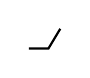
\begin{tikzpicture}[baseline=(current bounding box.south)]
        \draw[thick] (0,0) -- (0.25,0) -- (0.4,0.25);
    \end{tikzpicture}}}\!\!}

% Color definitions
\definecolor{kernelcolor}{RGB}{200,0,0}      % Red for K (kernels)
\definecolor{sobolevcolor}{RGB}{0,0,200}     % Blue for P (Sobolev)
\definecolor{theoremcolor}{RGB}{240,248,255} % Light blue for theorem boxes
\definecolor{definitioncolor}{RGB}{255,248,240} % Light orange for definitions

% Enhanced math commands
\newcommand{\E}{\mathbb{E}}
\DeclareMathOperator{\Var}{Var}
\newcommand{\indic}{\mathbb{1}}
\newcommand{\dd}{\,d}

% Colored operators
\newcommand{\Kop}{\textcolor{kernelcolor}{\mathbf{K}}}
\newcommand{\Pop}{\textcolor{sobolevcolor}{\mathbf{P}}}
\newcommand{\Kinf}{\textcolor{kernelcolor}{K^{\infty}}}
\newcommand{\Ps}{\textcolor{sobolevcolor}{P_s}}
\newcommand{\Ts}{\mathcal{T}_s}

% Beautiful theorem environments
\theoremstyle{plain}
\newtheorem{theorem}{Theorem}[section]
\newtheorem{lemma}[theorem]{Lemma}
\newtheorem{corollary}[theorem]{Corollary}
\newtheorem{proposition}[theorem]{Proposition}

\theoremstyle{definition}
\newtheorem{definition}[theorem]{Definition}
\newtheorem{example}[theorem]{Example}

\theoremstyle{remark}
\newtheorem*{remark}{Remark}

% Colored theorem boxes using tcolorbox
\tcolorboxenvironment{theorem}{
  colback=theoremcolor,
  colframe=blue!50!black,
  fonttitle=\bfseries,
  before skip=10pt,
  after skip=10pt,
  enhanced,
  drop shadow
}

\tcolorboxenvironment{definition}{
  colback=definitioncolor,
  colframe=orange!50!black,
  fonttitle=\bfseries,
  before skip=10pt,
  after skip=10pt,
  enhanced,
  drop shadow
}

\tcolorboxenvironment{lemma}{
  colback=green!5,
  colframe=green!50!black,
  fonttitle=\bfseries,
  before skip=8pt,
  after skip=8pt
}

\tcolorboxenvironment{corollary}{
  colback=purple!5,
  colframe=purple!50!black,
  fonttitle=\bfseries,
  before skip=8pt,
  after skip=8pt
}

\author{Janis AIAD}
\date{\today}
\title{Analysis of Deep Neural Network Learning Dynamics Through the NTK Lens}
\subtitle{Deeper or Wider ? A 1st answer under the NTK perspective}
% to change logo, add the image in PDF format
% or image by dragging it to the right and replace typographix
% with the image name, if you don't want a logo, 
% delete the line. 

\begin{figure*}[b]
    
\includegraphics[width=0.4\linewidth]{figures/umdlogo.jpg}
    \label{fig:enter-label}
\end{figure}


\fontsize{40pt}{48pt}

\begin{document}
	\maketitle 
	
	\tableofcontents
\newpage

\addcontentsline{toc}{section}{Abstract}
\section*{Abstract}
This report presents the results of a research internship focused on studying the learning dynamics of deep neural networks. We explore the underlying mechanisms through the Neural Tangent Kernel (NTK) formalism \cite{jacot2018neural}, with particular attention to finite-width corrections \cite{seleznova2022ntk_beyond}. Our work revolves around the decomposition of the NTK via Sobolev training, the analysis of its reproducing kernel Hilbert space (RKHS), and the study of extreme eigenvalues. We present theoretical bounds for the smallest eigenvalue of the NTK using random matrix theory (RMT) techniques. These results are then applied to analyze different architectures, including feed-forward neural networks (FCNN), matrix memory neural networks (MMNN), and transformers. We also discuss the implications of our findings for scientific machine learning (SciML) applications and propose directions for future research.

\newpage
\addcontentsline{toc}{section}{Executive summary}


\newpage
\addcontentsline{toc}{section}{Introduction}
\section*{Introduction}
The study of learning dynamics in deep neural networks constitutes a fundamental research area. Our approach focuses on the desingularization of Sobolev training by decomposing the problem into two distinct contributions: an independent neural tangent kernel (NTK) and a Sobolev contribution. This decomposition relies on the commutation between integral operators and the fractional Laplace operator.

\textbf{Key Discovery}: We establish that this commutation property holds \textit{exactly} only when using \textcolor{red}{\textbf{Chebyshev points}} (or equivalent optimal interpolation nodes) for sampling. For general sampling points, commutation breaks, necessitating explicit derivative information for effective learning. This fundamental distinction explains the empirical success of Physics-Informed Neural Networks (PINNs) and derivative-augmented methods over standard regression in most practical settings.

Our analysis continues with the study of NTK preconditioning through a freeze weights method, illustrated by neural networks factorizing low-rank weight matrices. This approach is supported by a rigorous approximation theorem. For classical feed-forward networks (FCNN), we develop a finite-width correction that proves particularly fruitful. Finally, we explore Transformers as an alternative solution, offering a new learning paradigm.

Across these different architectures, we study feature learning regimes and their scaling with network width. Our results rely on statistical physics tools to characterize model convergence and asymptotic behavior. This analysis enables a better understanding of finite-width corrections \cite{seleznova2022ntk_beyond} and their implications for the practical optimization of deep neural networks.


\newpage
\addcontentsline{toc}{section}{Notations}
\section*{Notations}

\begin{tcolorbox}[colback=blue!5,colframe=blue!50!black,title={\large \textbf{Mathematical Notation Reference}},enhanced,drop shadow]

\subsection*{Basic Mathematical Symbols}
\begin{longtable}{p{0.2\textwidth}p{0.15\textwidth}p{0.2\textwidth}p{0.15\textwidth}}
\toprule
\textbf{Symbol} & \textbf{Definition} & \textbf{Symbol} & \textbf{Definition} \\
\midrule
$\mathbb{R}$ & Set of real numbers & $\mathbb{N}$ & Set of natural numbers \\
$\mathbb{C}$ & Set of complex numbers & $\mathbb{S}^{d-1}$ & Unit sphere of dimension $d-1$ \\
$\E[\cdot]$ & Mathematical expectation & $\Var(\cdot)$ & Variance of a random variable \\
$\Cov(\cdot,\cdot)$ & Covariance between two variables & $\Corr(\cdot,\cdot)$ & Correlation between two variables \\
$\indic\{\cdot\}$ & Indicator function & $\dd x$ & Differential element \\
$\|\cdot\|$ & Euclidean norm & $\langle \cdot,\cdot \rangle$ & Inner product \\
$\mathcal{O}(\cdot)$ & Landau notation (big O) & $\tilde{\Omega}(\cdot)$ & Landau notation (big Omega tilde) \\
\bottomrule
\end{longtable}

\subsection*{Neural Network and Activation Functions}
\begin{longtable}{p{0.2\textwidth}p{0.15\textwidth}p{0.2\textwidth}p{0.15\textwidth}}
\toprule
\textbf{Symbol} & \textbf{Definition} & \textbf{Symbol} & \textbf{Definition} \\
\midrule
$\ReLU$ & ReLU activation function & $f(\mathbf{x}; \boldsymbol{\theta})$ & Neural network function \\
$\sigma(\cdot)$ & General activation function & $\sigma^2$ & Activation variance parameter \\
$L$ & Number of layers & $n_k$ & Width of layer $k$ \\
\bottomrule
\end{longtable}

\subsection*{Neural Tangent Kernel (NTK)}
\begin{longtable}{p{0.2\textwidth}p{0.15\textwidth}p{0.2\textwidth}p{0.15\textwidth}}
\toprule
\textbf{Symbol} & \textbf{Definition} & \textbf{Symbol} & \textbf{Definition} \\
\midrule
$\textcolor{kernelcolor}{\mathbf{K}}$ & Discrete NTK matrix & $\textcolor{kernelcolor}{K^{\infty}}$ & Infinite-width NTK operator \\
$K^{L}(\mathbf{x}_i, \mathbf{x}_j)$ & NTK for $L$-layer network & $\mu_\ell^{(K)}$ & NTK eigenvalues at degree $\ell$ \\
$\varrho(\rho)$ & Correlation propagation function & $\rho_1(\mathbf{x},\mathbf{x}')$ & Initial correlation \\
\bottomrule
\end{longtable}

\end{tcolorbox}

\begin{tcolorbox}[colback=blue!5,colframe=blue!50!black,title={\large \textbf{Mathematical Notation Reference}},enhanced,drop shadow]

\newpage
\subsection*{Sobolev Spaces and Training}
\begin{longtable}{p{0.2\textwidth}p{0.15\textwidth}p{0.2\textwidth}p{0.15\textwidth}}
\toprule
\textbf{Symbol} & \textbf{Definition} & \textbf{Symbol} & \textbf{Definition} \\
\midrule
$H^s(\Omega)$ & Sobolev space of order $s$ & $\textcolor{sobolevcolor}{\mathbf{P}}_s$ & Discrete Sobolev operator matrix \\
$P_s$ & Continuous Sobolev operator & $\mathcal{L}_{\text{Sobolev}}(f)$ & Sobolev training loss function \\
$D^k$ & $k$-th derivative operator & $\|f\|_{H^s}$ & Sobolev norm of order $s$ \\
$(I + (-\Delta)^{1/2})^s$ & Fractional Laplacian operator & $\Delta_{\mathbb{S}^{d-1}}$ & Laplace-Beltrami operator \\
\bottomrule
\end{longtable}

\subsection*{Spherical Harmonics and Fourier Analysis}
\begin{longtable}{p{0.2\textwidth}p{0.15\textwidth}p{0.2\textwidth}p{0.15\textwidth}}
\toprule
\textbf{Symbol} & \textbf{Definition} & \textbf{Symbol} & \textbf{Definition} \\
\midrule
$Y_{\ell,p}$ & Spherical harmonics & $N(d,\ell)$ & Multiplicity of harmonics \\
$\hat{f}(\xi)$ & Fourier transform of $f$ & $\xi$ & Frequency variable \\
$\sigma(x)$ & Surface measure on sphere & $\ell$ & Degree index \\
$p$ & Order index & $\nabla$ & Gradient operator \\
\bottomrule
\end{longtable}

\subsection*{Eigenvalues and Spectral Analysis}
\begin{longtable}{p{0.2\textwidth}p{0.15\textwidth}p{0.2\textwidth}p{0.15\textwidth}}
\toprule
\textbf{Symbol} & \textbf{Definition} & \textbf{Symbol} & \textbf{Definition} \\
\midrule
$\lambda_\ell$ & Eigenvalues at degree $\ell$ & $\lambda_{\min}(A)$ & Minimum eigenvalue \\
$\lambda_{\max}(A)$ & Maximum eigenvalue & $\mu_\ell^{(P_s)}$ & Sobolev eigenvalues \\
$C(d,L)$ & Constants depending on $d,L$ & $\Gamma(\cdot)$ & Gamma function \\
$P_\ell^{(\alpha)}(t)$ & Gegenbauer polynomials & $\tilde{K}_L^{\infty}(t)$ & Normalized NTK function \\
\bottomrule
\end{longtable}

\subsection*{Matrix Operations and Training}
\begin{longtable}{p{0.2\textwidth}p{0.15\textwidth}p{0.2\textwidth}p{0.15\textwidth}}
\toprule
\textbf{Symbol} & \textbf{Definition} & \textbf{Symbol} & \textbf{Definition} \\
\midrule
$A^T$ & Matrix transpose & $\|A\|_{op}$ & Operator norm \\
$\|A\|_F$ & Frobenius norm & $A \circ B$ & Hadamard product \\
$\mathcal{T}_s$ & Composite learning operator & $a_{\ell,p}$ & Sampling vectors \\
$\eta$ & Learning rate & $f_t(x)$ & Network at time $t$ \\
$y_i$ & Target output & $n$ & Number of samples \\
$d$ & Input dimension & $s$ & Sobolev order \\
\bottomrule
\end{longtable}

\end{tcolorbox}

\newpage




\section{Corrections à Largeur Finie et Régimes d'Apprentissage}

\subsection{Développement Théorique pour les FCNN}
(Présentation des théorèmes et formules pour les corrections à largeur finie dans les FCNN. Analyse des lois de scaling du reste et discussion sur les termes d'erreur, en lien avec les ensembles de matrices aléatoires QUE & GOE.)



\section{Framework and Notations}

In this section, we introduce the mathematical framework and notations used throughout this document, building upon the definitions established in the work on the Neural Tangent Hierarchy (NTH) \cite{dyer2019asymptoticswidenetworksfeynman}.

\subsection{Neural Network Architecture}

We consider a fully-connected feedforward neural network with $H$ hidden layers of width $m$.
\begin{itemize}
    \item The network input is a vector $x \in \mathbb{R}^d$.
    \item The output of layer $\ell$ is denoted by $x^{(\ell)}$. For $\ell \in \{1, \dots, H\}$, it is computed recursively as:
    \begin{equation}
        x^{(\ell)} = \frac{1}{\sqrt{m}}\sigma(W^{(\ell)}x^{(\ell-1)})
    \end{equation}
    where $x^{(0)} = x$ is the input, $W^{(\ell)}$ is the weight matrix of layer $\ell$, and $\sigma$ is a non-linear activation function applied component-wise.
    \item The final output of the network is a linear combination of the last hidden layer's output:
    \begin{equation}
        f(x, \theta) = a^T x^{(H)}
    \end{equation}
    where $a \in \mathbb{R}^m$ is the weight vector of the output layer.
    \item The set of all trainable parameters of the network is denoted $\theta = (\text{vec}(W^{(1)}), \dots, \text{vec}(W^{(H)}), a)$.
    \item The derivative of the activation function for layer $\ell$ is represented by a diagonal matrix $\sigma'_\ell(x) = \text{diag}(\sigma'(W^{(\ell)}x^{(\ell-1)}))$.
\end{itemize}

\subsection{The Neural Tangent Kernel (NTK)}

The network is trained via gradient descent on the quadratic loss: $L(\theta) = \frac{1}{2n}\sum_{\alpha=1}^n (f(x_\alpha, \theta) - y_\alpha)^2$. The dynamics of the network function $f(x, \theta_t)$ during continuous-time training (gradient flow) are governed by the Neural Tangent Kernel (NTK), denoted $K^{(2)}_t$.
\begin{equation}
\frac{d}{dt} f(x, \theta_t) = -\frac{1}{n}\sum_{\beta=1}^n K^{(2)}_t(x, x_\beta) (f(x_\beta, \theta_t) - y_\beta)
\end{equation}
The NTK is defined as the inner product of the gradients of the output function with respect to the network parameters:
\begin{equation}
K^{(2)}_t(x_\alpha, x_\beta) := \langle \nabla_\theta f(x_\alpha, \theta_t), \nabla_\theta f(x_\beta, \theta_t) \rangle
\end{equation}
It can be decomposed as a sum over the network layers:
\begin{equation}
K^{(2)}_t(x_\alpha, x_\beta) = \langle x^{(H)}_\alpha, x^{(H)}_\beta \rangle + \sum_{\ell=1}^{H} \langle G^{(\ell)}_\alpha, G^{(\ell)}_\beta \rangle \langle x^{(\ell-1)}_\alpha, x^{(\ell-1)}_\beta \rangle
\end{equation}
where the vector $G^{(\ell)}_\mu$ represents the backpropagated gradient up to layer $\ell$:
\begin{equation}
G^{(\ell)}_\mu = \frac{1}{\sqrt{m}}\sigma'_\ell(x_\mu) (W^{(\ell+1)})^T \cdots \frac{1}{\sqrt{m}}\sigma'_H(x_\mu) a_t
\end{equation}

\subsection{The Neural Tangent Hierarchy (NTH)}
For finite-width networks ($m < \infty$), the NTK $K^{(2)}_t$ is not constant but evolves during training. Its dynamics are dictated by the higher-order kernel $K^{(3)}_t$. This gives rise to an infinite sequence of coupled ordinary differential equations, known as the Neural Tangent Hierarchy (NTH):
\begin{equation}
\frac{d}{dt} K^{(r)}_t(x_{\alpha_1}, \dots, x_{\alpha_r}) = -\frac{1}{n} \sum_{\gamma=1}^n K^{(r+1)}_t(x_{\alpha_1}, \dots, x_{\alpha_r}, x_\gamma) (f_t(x_\gamma) - y_\gamma)
\end{equation}
valid for all $r \ge 2$. The higher-order kernel $K^{(r+1)}$ is defined recursively as the derivative of $K^{(r)}$ with respect to the parameters, contracted with the gradient of the network output:
\begin{equation}
K^{(r+1)}_t(x_1, \dots, x_{r+1}) := \langle \nabla_\theta K^{(r)}_t(x_1, \dots, x_r), \nabla_\theta f_t(x_{r+1}) \rangle
\end{equation}
This hierarchy captures the complete training dynamics beyond the infinite-width approximation where only $K^{(2)}$ is considered and is constant. The purpose of this document is to derive and analyze the explicit form of $K^{(3)}$, which represents the first correction to the NTK dynamics.

\section{Other proof}

In the framework of the Neural Tangent Hierarchy (NTH), the kernel $K^{(3)}$ arises as the operator governing the time evolution of the Neural Tangent Kernel $K^{(2)}$. The dynamics of $K^{(2)}$ under gradient flow are given by:
\begin{equation}
\frac{d}{dt} K^{(2)}_t(x_\alpha, x_\beta) = -\frac{1}{n} \sum_{\gamma=1}^n K^{(3)}_t(x_\alpha, x_\beta, x_\gamma) (f_t(x_\gamma) - y_\gamma)
\end{equation}
where $K^{(3)}_t(x_\alpha, x_\beta, x_\gamma)$ is defined as the contraction of the gradient of $K^{(2)}_t(x_\alpha, x_\beta)$ with respect to the network parameters $\theta$ with the gradient of the network output $f_t(x_\gamma)$:
\begin{equation}
K^{(3)}_t(x_\alpha, x_\beta, x_\gamma) := \langle \nabla_\theta K^{(2)}_t(x_\alpha, x_\beta), \nabla_\theta f_t(x_\gamma) \rangle.
\end{equation}

Let's derive the explicit formula for $K^{(3)}_t$. We start from the expression for $K^{(2)}_t(x_\alpha, x_\beta)$:
\begin{equation}
K^{(2)}_t(x_\alpha, x_\beta) = \langle x^{(H)}_\alpha, x^{(H)}_\beta \rangle + \sum_{\ell=1}^{H} \langle G^{(\ell)}_\alpha, G^{(\ell)}_\beta \rangle \langle x^{(\ell-1)}_\alpha, x^{(\ell-1)}_\beta \rangle
\end{equation}
where we use the notation:
\begin{itemize}
    \item $x^{(p)}_\mu = \frac{1}{\sqrt{m}}\sigma(W^{(p)} x^{(p-1)}_\mu)$ for $p \ge 1$, and $x^{(0)}_\mu = x_\mu$.
    \item $G^{(\ell)}_\mu = \frac{1}{\sqrt{m}}\sigma'_\ell(x_\mu) (W^{(\ell+1)})^T \cdots \frac{1}{\sqrt{m}}\sigma'_H(x_\mu) a_t$, with $\sigma'_\ell(x_\mu) = \text{diag}(\sigma'(W^{(\ell)}x^{(\ell-1)}_\mu))$.
\end{itemize}

Let $\delta_\gamma(\cdot) := \langle \nabla_\theta (\cdot), \nabla_\theta f_t(x_\gamma) \rangle$ denote the directional derivative along $\nabla_\theta f_t(x_\gamma)$. Then $K^{(3)}_{\alpha\beta\gamma} = \delta_\gamma(K^{(2)}_{\alpha\beta})$. Applying the product rule, we get:
\begin{align}
K^{(3)}_{\alpha\beta\gamma} = \delta_\gamma \langle x^{(H)}_\alpha, x^{(H)}_\beta \rangle + \sum_{\ell=1}^{H} \delta_\gamma \left( \langle G^{(\ell)}_\alpha, G^{(\ell)}_\beta \rangle \langle x^{(\ell-1)}_\alpha, x^{(\ell-1)}_\beta \rangle \right)
\end{align}
Each term expands further, following $\delta_\gamma \langle A, B \rangle = \langle \delta_\gamma A, B \rangle + \langle A, \delta_\gamma B \rangle$. This results in a sum over all components of $K^{(2)}_{\alpha\beta}$, where each component is acted upon by $\delta_\gamma$. The core of the derivation lies in computing $\delta_\gamma$ for the building blocks $x^{(p)}_\mu$ and $G^{(p)}_\mu$.

The recursive formula for the derivative of the activations is:
\begin{equation}
\delta_\gamma x^{(p)}_\mu = \frac{1}{\sqrt{m}} \sigma'_{p}(x_\mu) \left( W^{(p)} (\delta_\gamma x^{(p-1)}_\mu) + \langle x^{(p-1)}_\gamma, x^{(p-1)}_\mu \rangle G^{(p)}_\gamma \right)
\end{equation}
with the base case $\delta_\gamma x^{(0)}_\mu = \delta_\gamma x_\mu = 0$.

The derivative of the backpropagated vectors $G^{(\ell)}_\mu$ is given by a sum of terms, where $\delta_\gamma$ acts on one factor at a time:
\begin{align}
\delta_\gamma G^{(\ell)}_\mu = \sum_{p=\ell}^{H} & \left( \frac{1}{\sqrt{m}}\sigma'_\ell(x_\mu) \cdots \delta_\gamma(\frac{1}{\sqrt{m}}(W^{(p+1)})^T) \cdots \sigma'_H(x_\mu) a_t \right) \\
+ \sum_{p=\ell}^{H} & \left( \frac{1}{\sqrt{m}}\sigma'_\ell(x_\mu) \cdots \delta_\gamma(\sigma'_{p}(x_\mu)) \cdots \sigma'_H(x_\mu) a_t \right) \\
+ & \left( \frac{1}{\sqrt{m}}\sigma'_\ell(x_\mu) \cdots \sigma'_H(x_\mu) (\delta_\gamma a_t) \right)
\end{align}
where
\begin{itemize}
    \item $\delta_\gamma a_t = x^{(H)}_\gamma$
    \item The term $\delta_\gamma((W^{(p+1)})^T)$ corresponds to a rank-1 update which, when contracted in context, yields terms involving $G^{(p+1)}_\gamma$ and inner products of activations.
    \item $\delta_\gamma(\sigma'_{p}(x_\mu)) = \sigma''_{p}(x_\mu) \text{diag}(\delta_\gamma(W^{(p)}x^{(p-1)}_\mu/\sqrt{m}))$. This term vanishes for ReLU activation functions as $\sigma''=0$ almost everywhere.
\end{itemize}

Combining these rules gives the complete formula for $K^{(3)}_t(x_\alpha, x_\beta, x_\gamma)$. It is a sum of many terms, each corresponding to differentiating one part of $K^{(2)}_t(x_\alpha, x_\beta)$. For clarity, we write it as a sum of contributions:
\begin{equation}
K^{(3)}_{\alpha\beta\gamma} = K^{(3, \text{out})}_{\alpha\beta\gamma} + \sum_{\ell=1}^H \left( K^{(3, G)}_{\alpha\beta\gamma, \ell} + K^{(3, x)}_{\alpha\beta\gamma, \ell} \right)
\end{equation}
where
\begin{align}
K^{(3, \text{out})}_{\alpha\beta\gamma} &= \langle \delta_\gamma x^{(H)}_\alpha, x^{(H)}_\beta \rangle + \langle x^{(H)}_\alpha, \delta_\gamma x^{(H)}_\beta \rangle \\
K^{(3, G)}_{\alpha\beta\gamma, \ell} &= \left( \langle \delta_\gamma G^{(\ell)}_\alpha, G^{(\ell)}_\beta \rangle + \langle G^{(\ell)}_\alpha, \delta_\gamma G^{(\ell)}_\beta \rangle \right) \langle x^{(\ell-1)}_\alpha, x^{(\ell-1)}_\beta \rangle \\
K^{(3, x)}_{\alpha\beta\gamma, \ell} &= \langle G^{(\ell)}_\alpha, G^{(\ell)}_\beta \rangle \left( \langle \delta_\gamma x^{(\ell-1)}_\alpha, x^{(\ell-1)}_\beta \rangle + \langle x^{(\ell-1)}_\alpha, \delta_\gamma x^{(\ell-1)}_\beta \rangle \right)
\end{align}
The terms $\delta_\gamma x^{(p)}_\mu$ and $\delta_\gamma G^{(p)}_\mu$ are expanded using the recursive rules above, yielding a full, albeit lengthy, expression. This hierarchical structure is characteristic of the NTH framework.


\section{Extended Formula for $K^{(3)}$}

To obtain a complete expression for $K^{(3)}_{\alpha\beta\gamma}$, we expand the terms $\delta_\gamma x^{(p)}_\mu$ and $\delta_\gamma G^{(\ell)}_\mu$ using their recursive definitions. We assume a ReLU activation function, so $\sigma''=0$ almost everywhere.

\subsection{Development of Recursive Terms}

The term $\delta_\gamma x^{(p)}_\mu$, which represents the variation of activation $x^{(p)}_\mu$ along the gradient of output $f_t(x_\gamma)$, can be expanded as a sum over previous layers:
\begin{equation}
\delta_\gamma x^{(p)}_\mu = \sum_{j=1}^{p} \left( \prod_{k=j+1}^{p} \frac{\sigma'_{k}(x_\mu) W^{(k)}}{\sqrt{m}} \right) \frac{\sigma'_{j}(x_\mu)}{\sqrt{m}} \langle x^{(j-1)}_\gamma, x^{(j-1)}_\mu \rangle G^{(j)}_\gamma
\end{equation}
where the product $\prod_{k=j+1}^{p}$ is an ordered product of Jacobian matrices.

Similarly, the term $\delta_\gamma G^{(\ell)}_\mu$, the variation of the backpropagated gradient vector, decomposes into a sum over subsequent layers:
\begin{align}
\delta_\gamma G^{(\ell)}_\mu = & \sum_{p=\ell}^{H-1} \left( \prod_{k=\ell}^{p} \frac{(W^{(k+1)})^T \sigma'_{k+1}(x_\mu)}{\sqrt{m}} \right) \frac{1}{m} G^{(p+1)}_\gamma \langle x^{(p)}_\gamma, x^{(p)}_\mu \rangle \\
& + \left( \prod_{k=\ell}^{H-1} \frac{(W^{(k+1)})^T \sigma'_{k+1}(x_\mu)}{\sqrt{m}} \right) \frac{x^{(H)}_\gamma}{\sqrt{m}}
\end{align}
The first term captures the effect of varying weights $W^{(\ell+1)}, \dots, W^{(H)}$, and the second term that of varying the output vector $a_t$.

\subsection{Complete Expression}

Substituting these expressions into equations (18), (19) and (20) yields the complete formula for $K^{(3)}_{\alpha\beta\gamma}$. It is a sum of $2H^2 + 2H$ terms.
\begin{align}
K^{(3)}_{\alpha\beta\gamma} = & \sum_{j=1}^{H} \left( \langle \mathcal{J}^{(H \to j)}_{\alpha} \mathcal{T}^{(j)}_{\gamma\alpha}, x^{(H)}_\beta \rangle + \langle x^{(H)}_\alpha, \mathcal{J}^{(H \to j)}_{\beta} \mathcal{T}^{(j)}_{\gamma\beta} \rangle \right) \nonumber \\
& + \sum_{\ell=1}^{H} \langle x^{(\ell-1)}_\alpha, x^{(\ell-1)}_\beta \rangle \sum_{p=\ell}^{H-1} \left( \langle \mathcal{B}^{(\ell \to p)}_{\alpha} \mathcal{U}^{(p)}_{\gamma\alpha}, G^{(\ell)}_\beta \rangle + \langle G^{(\ell)}_\alpha, \mathcal{B}^{(\ell \to p)}_{\beta} \mathcal{U}^{(p)}_{\gamma\beta} \rangle \right) \nonumber \\
& + \sum_{\ell=1}^{H} \langle x^{(\ell-1)}_\alpha, x^{(\ell-1)}_\beta \rangle \left( \langle \mathcal{B}^{(\ell \to H-1)}_{\alpha} \frac{x^{(H)}_\gamma}{\sqrt{m}}, G^{(\ell)}_\beta \rangle + \langle G^{(\ell)}_\alpha, \mathcal{B}^{(\ell \to H-1)}_{\beta} \frac{x^{(H)}_\gamma}{\sqrt{m}} \rangle \right) \nonumber \\
& + \sum_{\ell=1}^{H} \langle G^{(\ell)}_\alpha, G^{(\ell)}_\beta \rangle \sum_{j=1}^{\ell-1} \left( \langle \mathcal{J}^{(\ell-1 \to j)}_{\alpha} \mathcal{T}^{(j)}_{\gamma\alpha}, x^{(\ell-1)}_\beta \rangle + \langle x^{(\ell-1)}_\alpha, \mathcal{J}^{(\ell-1 \to j)}_{\beta} \mathcal{T}^{(j)}_{\gamma\beta} \rangle \right)
\end{align}
where we have defined for readability:
\begin{itemize}
    \item Forward propagators (Jacobian): $\mathcal{J}^{(p \to j)}_{\mu} = \prod_{k=j+1}^{p} \frac{\sigma'_{k}(x_\mu) W^{(k)}}{\sqrt{m}}$
    \item Forward source terms: $\mathcal{T}^{(j)}_{\gamma\mu} = \frac{\sigma'_{j}(x_\mu)}{\sqrt{m}} \langle x^{(j-1)}_\gamma, x^{(j-1)}_\mu \rangle G^{(j)}_\gamma$
    \item Backward propagators: $\mathcal{B}^{(\ell \to p)}_{\mu} = \prod_{k=\ell}^{p} \frac{(W^{(k+1)})^T \sigma'_{k+1}(x_\mu)}{\sqrt{m}}$
    \item Backward source terms: $\mathcal{U}^{(p)}_{\gamma\mu} = \frac{1}{m} G^{(p+1)}_\gamma \langle x^{(p)}_\gamma, x^{(p)}_\mu \rangle$
\end{itemize}
This formula, while complex, represents the complete hierarchical structure of the first-order correction to the NTK dynamics.

\section{Fully Expanded Non-Recursive Formula for $K^{(3)}$}

Here, we present the complete, non-recursive expression for $K^{(3)}_{\alpha\beta\gamma}$. This formula is obtained by substituting the expanded expressions for the directional derivatives $\delta_\gamma x^{(p)}_\mu$ and $\delta_\gamma G^{(\ell)}_\mu$ into the decomposed formula for $K^{(3)}$. This makes the dependency on the network parameters (weights $W^{(k)}$ and output vectors $a_t$) and activations at each layer fully explicit. We continue to assume a ReLU activation function, which sets second derivatives of $\sigma$ to zero almost everywhere.

The final expression is a sum of four main components, corresponding to the differentiation of the output layer activations, the backward vectors, and the hidden layer activations:

\begin{align}
K^{(3)}_{\alpha\beta\gamma} = & \nonumber \\
% K^(3,out) term
& \sum_{j=1}^{H} \Biggl( \left\langle \left( \prod_{k=j+1}^{H} \frac{\sigma'_{k}(x_\alpha) W^{(k)}}{\sqrt{m}} \right) \frac{\sigma'_{j}(x_\alpha)}{\sqrt{m}} \langle x^{(j-1)}_\gamma, x^{(j-1)}_\alpha \rangle G^{(j)}_\gamma, x^{(H)}_\beta \right\rangle \nonumber \\
& \quad + \left\langle x^{(H)}_\alpha, \left( \prod_{k=j+1}^{H} \frac{\sigma'_{k}(x_\beta) W^{(k)}}{\sqrt{m}} \right) \frac{\sigma'_{j}(x_\beta)}{\sqrt{m}} \langle x^{(j-1)}_\gamma, x^{(j-1)}_\beta \rangle G^{(j)}_\gamma \right\rangle \Biggr) \nonumber \\
% K^(3,G) term
& + \sum_{\ell=1}^{H} \langle x^{(\ell-1)}_\alpha, x^{(\ell-1)}_\beta \rangle \Biggl[ \nonumber \\
& \quad \sum_{p=\ell}^{H-1} \Biggl( \left\langle \left( \prod_{k=\ell}^{p} \frac{(W^{(k+1)})^T \sigma'_{k+1}(x_\alpha)}{\sqrt{m}} \right) \frac{G^{(p+1)}_\gamma \langle x^{(p)}_\gamma, x^{(p)}_\alpha \rangle}{m}, G^{(\ell)}_\beta \right\rangle \nonumber \\
& \qquad + \left\langle G^{(\ell)}_\alpha, \left( \prod_{k=\ell}^{p} \frac{(W^{(k+1)})^T \sigma'_{k+1}(x_\beta)}{\sqrt{m}} \right) \frac{G^{(p+1)}_\gamma \langle x^{(p)}_\gamma, x^{(p)}_\beta \rangle}{m} \right\rangle \Biggr) \nonumber \\
& \quad + \left\langle \left( \prod_{k=\ell}^{H-1} \frac{(W^{(k+1)})^T \sigma'_{k+1}(x_\alpha)}{\sqrt{m}} \right) \frac{x^{(H)}_\gamma}{\sqrt{m}}, G^{(\ell)}_\beta \right\rangle \nonumber \\
& \quad + \left\langle G^{(\ell)}_\alpha, \left( \prod_{k=\ell}^{H-1} \frac{(W^{(k+1)})^T \sigma'_{k+1}(x_\beta)}{\sqrt{m}} \right) \frac{x^{(H)}_\gamma}{\sqrt{m}} \right\rangle \Biggr] \nonumber \\
% K^(3,x) term
& + \sum_{\ell=1}^{H} \langle G^{(\ell)}_\alpha, G^{(\ell)}_\beta \rangle \sum_{j=1}^{\ell-1} \Biggl( \left\langle \left( \prod_{k=j+1}^{\ell-1} \frac{\sigma'_{k}(x_\alpha) W^{(k)}}{\sqrt{m}} \right) \frac{\sigma'_{j}(x_\alpha)}{\sqrt{m}} \langle x^{(j-1)}_\gamma, x^{(j-1)}_\alpha \rangle G^{(j)}_\gamma, x^{(\ell-1)}_\beta \right\rangle \nonumber \\
& \quad + \left\langle x^{(\ell-1)}_\alpha, \left( \prod_{k=j+1}^{\ell-1} \frac{\sigma'_{k}(x_\beta) W^{(k)}}{\sqrt{m}} \right) \frac{\sigma'_{j}(x_\beta)}{\sqrt{m}} \langle x^{(j-1)}_\gamma, x^{(j-1)}_\beta \rangle G^{(j)}_\gamma \right\rangle \Biggr)
\end{align}
In this expression, the products $\prod$ represent ordered matrix products. The empty product $\prod_{k=p+1}^p$ is defined as the identity matrix. This detailed formula lays bare the intricate dependencies of the NTK dynamics on the network's architecture and parameters at finite width.


\newpage


\section{Recursive Formula for $K^{(3)}$ as a Function of Depth $H$}

To analyze the influence of network depth, it is useful to establish a recursive relation for $K^{(3)}$. Let $K^{(3, H)}_{\alpha\beta\gamma}$ denote the kernel for a network with $H$ layers. The goal is to express $K^{(3, H+1)}_{\alpha\beta\gamma}$ in terms of quantities computed for a network with $H$ layers.

The starting point is the decomposition of $K^{(2, H+1)}_{\alpha\beta}$, the NTK for a network with $H+1$ layers:
\begin{equation}
K^{(2, H+1)}_{\alpha\beta} = \underbrace{\left( \langle x^{(H)}_\alpha, x^{(H)}_\beta \rangle + \sum_{\ell=1}^{H} \langle G'^{(\ell)}_\alpha, G'^{(\ell)}_\beta \rangle \langle x^{(\ell-1)}_\alpha, x^{(\ell-1)}_\beta \rangle \right)}_{K^{(2,H)}_{\alpha\beta} \text{ with } a'_t} + T_{H+1} + C_{H+1}
\end{equation}
where:
\begin{itemize}
    \item $x^{(H+1)}_\mu = \frac{1}{\sqrt{m}}\sigma(W^{(H+1)} x^{(H)}_\mu)$.
    \item $a'_t = \frac{1}{\sqrt{m}} (W^{(H+1)})^T \sigma'_{H+1} a_t$ is an "effective output vector" that replaces $a_t$ in the computations of $G^{(\ell)}$ for $\ell \le H$.
    \item $T_{H+1} = \langle G^{(H+1)}_\alpha, G^{(H+1)}_\beta \rangle \langle x^{(H)}_\alpha, x^{(H)}_\beta \rangle$ is the term from the new layer $H+1$.
    \item $C_{H+1} = \langle x^{(H+1)}_\alpha, x^{(H+1)}_\beta \rangle - \langle a'_t, a'_t \rangle \langle x^{(H)}_\alpha, x^{(H)}_\beta \rangle$ is a correction term.
\end{itemize}
The vectors $G'^{(\ell)}$ are the backpropagated gradients in a network with $H$ layers but with $a'_t$ as output weights, while $G^{(H+1)}$ is the gradient for layer $H+1$.

Applying the directional derivative operator $\delta_\gamma(\cdot) = \langle \nabla_\theta (\cdot), \nabla_\theta f_t(x_\gamma) \rangle$, we obtain the recursion for $K^{(3)}$:
\begin{equation}
K^{(3, H+1)}_{\alpha\beta\gamma} = \delta_\gamma \left(K^{(2,H)}_{\alpha\beta, a'_t} \right) + \delta_\gamma(T_{H+1}) + \delta_\gamma(C_{H+1})
\end{equation}
The term $\delta_\gamma \left(K^{(2,H)}_{\alpha\beta, a'_t} \right)$ is analogous to $K^{(3,H)}_{\alpha\beta\gamma}$, but with additional dependencies through $a'_t$. The other terms expand as follows:
\begin{align}
\delta_\gamma(T_{H+1}) &= \langle \delta_\gamma G^{(H+1)}_\alpha, G^{(H+1)}_\beta \rangle \langle x^{(H)}_\alpha, x^{(H)}_\beta \rangle + \dots \\
\delta_\gamma(C_{H+1}) &= \langle \delta_\gamma x^{(H+1)}_\alpha, x^{(H+1)}_\beta \rangle - \langle \delta_\gamma a'_t, a'_t \rangle \langle x^{(H)}_\alpha, x^{(H)}_\beta \rangle + \dots
\end{align}
This decomposition allows us to separate the effect of adding a layer by isolating terms specific to the new layer $(T_{H+1}, C_{H+1})$ and the modification of previous layer terms through $a'_t$.






\section{Framework and Notations}

In this section, we introduce the mathematical framework and notations used throughout this document, building upon the definitions established in the work on the Neural Tangent Hierarchy (NTH) \cite{dyer2019asymptoticswidenetworksfeynman}.

\subsection{Neural Network Architecture}

We consider a fully-connected feedforward neural network with $H$ hidden layers of width $m$.
\begin{itemize}
    \item The network input is a vector $x \in \mathbb{R}^d$.
    \item The output of layer $\ell$ is denoted by $x^{(\ell)}$. For $\ell \in \{1, \dots, H\}$, it is computed recursively as:
    \begin{equation}
        x^{(\ell)} = \frac{1}{\sqrt{m}}\sigma(W^{(\ell)}x^{(\ell-1)})
    \end{equation}
    where $x^{(0)} = x$ is the input, $W^{(\ell)}$ is the weight matrix of layer $\ell$, and $\sigma$ is a non-linear activation function applied component-wise.
    \item The final output of the network is a linear combination of the last hidden layer's output:
    \begin{equation}
        f(x, \theta) = a^T x^{(H)}
    \end{equation}
    where $a \in \mathbb{R}^m$ is the weight vector of the output layer.
    \item The set of all trainable parameters of the network is denoted $\theta = (\text{vec}(W^{(1)}), \dots, \text{vec}(W^{(H)}), a)$.
    \item The derivative of the activation function for layer $\ell$ is represented by a diagonal matrix $\sigma'_\ell(x) = \text{diag}(\sigma'(W^{(\ell)}x^{(\ell-1)}))$.
\end{itemize}

\subsection{The Neural Tangent Kernel (NTK)}

The network is trained via gradient descent on the quadratic loss: $L(\theta) = \frac{1}{2n}\sum_{\alpha=1}^n (f(x_\alpha, \theta) - y_\alpha)^2$. The dynamics of the network function $f(x, \theta_t)$ during continuous-time training (gradient flow) are governed by the Neural Tangent Kernel (NTK), denoted $K^{(2)}_t$.
\begin{equation}
\frac{d}{dt} f(x, \theta_t) = -\frac{1}{n}\sum_{\beta=1}^n K^{(2)}_t(x, x_\beta) (f(x_\beta, \theta_t) - y_\beta)
\end{equation}
The NTK is defined as the inner product of the gradients of the output function with respect to the network parameters:
\begin{equation}
K^{(2)}_t(x_\alpha, x_\beta) := \langle \nabla_\theta f(x_\alpha, \theta_t), \nabla_\theta f(x_\beta, \theta_t) \rangle
\end{equation}
It can be decomposed as a sum over the network layers:
\begin{equation}
K^{(2)}_t(x_\alpha, x_\beta) = \langle x^{(H)}_\alpha, x^{(H)}_\beta \rangle + \sum_{\ell=1}^{H} \langle G^{(\ell)}_\alpha, G^{(\ell)}_\beta \rangle \langle x^{(\ell-1)}_\alpha, x^{(\ell-1)}_\beta \rangle
\end{equation}
where the vector $G^{(\ell)}_\mu$ represents the backpropagated gradient up to layer $\ell$:
\begin{equation}
G^{(\ell)}_\mu = \frac{1}{\sqrt{m}}\sigma'_\ell(x_\mu) (W^{(\ell+1)})^T \cdots \frac{1}{\sqrt{m}}\sigma'_H(x_\mu) a_t
\end{equation}

\subsection{The Neural Tangent Hierarchy (NTH)}
For finite-width networks ($m < \infty$), the NTK $K^{(2)}_t$ is not constant but evolves during training. Its dynamics are dictated by the higher-order kernel $K^{(3)}_t$. This gives rise to an infinite sequence of coupled ordinary differential equations, known as the Neural Tangent Hierarchy (NTH):
\begin{equation}
\frac{d}{dt} K^{(r)}_t(x_{\alpha_1}, \dots, x_{\alpha_r}) = -\frac{1}{n} \sum_{\gamma=1}^n K^{(r+1)}_t(x_{\alpha_1}, \dots, x_{\alpha_r}, x_\gamma) (f_t(x_\gamma) - y_\gamma)
\end{equation}
valid for all $r \ge 2$. The higher-order kernel $K^{(r+1)}$ is defined recursively as the derivative of $K^{(r)}$ with respect to the parameters, contracted with the gradient of the network output:
\begin{equation}
K^{(r+1)}_t(x_1, \dots, x_{r+1}) := \langle \nabla_\theta K^{(r)}_t(x_1, \dots, x_r), \nabla_\theta f_t(x_{r+1}) \rangle
\end{equation}
This hierarchy captures the complete training dynamics beyond the infinite-width approximation where only $K^{(2)}$ is considered and is constant. The purpose of this document is to derive and analyze the explicit form of $K^{(3)}$, which represents the first correction to the NTK dynamics.

\section{Introduction}

This document analyzes the behavior of the entries of the $K^{(3)}$ tensor as a function of the network depth, denoted by $L$ (or $H$ in the code), for a fixed network width $m$. The analysis is based on the formulas from the Neural Tangent Hierarchy (NTH) framework. We aim to understand if the tensor entries decay as the depth increases, and specifically, if this decay is exponential.

\section{Scaling of Core Components in the NTK Formalism}

We consider a Multi-Layer Perceptron (MLP) of depth $L$ and uniform width $m$. The weights $W^{(\ell)}$ for $\ell=1, \dots, L$ are $m \times m$ matrices, and the output weights $a$ are in $\mathbb{R}^m$. We use the NTK scaling, where weights are initialized i.i.d. from a distribution with variance $c_W^2/m$ (e.g., $\mathcal{N}(0, c_W^2/m)$). The output layer is scaled by $1/\sqrt{m}$.

The forward activations $x^{(p)}_\mu$ and backward propagated vectors $G^{(\ell)}_\mu$ are the building blocks of the NTK.
The activations are defined as $x^{(p)}_\mu = \frac{1}{\sqrt{m}}\sigma(W^{(p)} x^{(p-1)}_\mu)$. With proper initialization ($c_W^2=2$ for ReLU), the norm of the activations is stable across layers:
\begin{equation}
    \mathbb{E}[\|x^{(p)}_\mu\|^2] \approx \|x^{(p-1)}_\mu\|^2
\end{equation}
Thus, we assume $\|x^{(p)}_\mu\| \sim O(1)$ for all layers $p$.

The backward vectors $G^{(\ell)}_\mu$ are defined recursively:
\begin{align}
    G^{(L)}_\mu &= \frac{a}{\sqrt{m}} \\
    G^{(\ell)}_\mu &= \frac{(W^{(\ell+1)})^T}{\sqrt{m}} \sigma'_{\ell+1}(x_\mu) G^{(\ell+1)}_\mu
\end{align}
where $\sigma'_{\ell+1}$ is the diagonal matrix of activation derivatives. A crucial point is to analyze the norm of the propagation operator $\mathcal{P}_\ell = \frac{(W^{(\ell+1)})^T}{\sqrt{m}} \sigma'_{\ell+1}(x_\mu)$. Based on random matrix theory, for a large matrix $W$ with i.i.d. entries of variance $\sigma_w^2$, its operator norm $\|W\|_{\text{op}}$ converges to $2\sigma_w\sqrt{m}$. Thus, the norm of our scaled operator is:
\begin{equation}
    \|\mathcal{P}_\ell\|_{\text{op}} \le \left\| \frac{W^{(\ell+1)}}{\sqrt{m}} \right\|_{\text{op}} \xrightarrow{m\to\infty} 2\sigma_w
\end{equation}
For standard initialization schemes (e.g., He initialization with $\sigma_w^2=2/m_{in}$), this value is $O(1)$ but not necessarily less than 1. A naive application of the sub-multiplicative property might suggest an exponential explosion of norms, as $\|G^{(\ell)}\| \le (2\sigma_w)^{L-\ell} \|G^{(L)}\|$.

However, this reasoning is flawed because we are multiplying a sequence of \textbf{independent} random matrices. The vector $G^{(\ell+1)}_\mu$, after being transformed by $\mathcal{P}_\ell$, is not aligned with the direction of maximal amplification of the next operator $\mathcal{P}_{\ell-1}$. The theory of products of random matrices shows that for deep networks, the norm is preserved on average if the initialization is chosen correctly to achieve a state of "dynamical isometry". This ensures that the system avoids both exponential explosion and vanishing of the signal. Therefore, we can confidently assume that the norms are stable across layers:
\begin{equation}
    \|G^{(\ell)}_\mu\| \sim O(1) \quad \text{for all } \ell
\end{equation}
These vectors do not exhibit a systematic decay or growth with depth.

\section{Analysis of the $K^{(3)}$ Tensor}

The $K^{(3)}$ tensor is constructed from the directional derivatives of $x^{(p)}_\mu$ and $G^{(\ell)}_\mu$, denoted $\delta_\gamma x^{(p)}_\mu$ and $\delta_\gamma G^{(\ell)}_\mu$.

\subsection{Forward Derivative Term $\delta_\gamma x^{(p)}_\mu$}

The recursive formula for $\delta_\gamma x^{(p)}_\mu$ is:
\begin{equation}
    \delta_\gamma x^{(p)}_\mu = \frac{1}{\sqrt{m}} \sigma'_{p}(x_\mu) \left( W^{(p)} (\delta_\gamma x^{(p-1)}_\mu) + \langle x^{(p-1)}_\gamma, x^{(p-1)}_\mu \rangle G^{(p)}_\gamma \right)
\end{equation}
with $\delta_\gamma x^{(0)}_\mu = 0$. Analyzing the norm:
\begin{equation}
    \|\delta_\gamma x^{(p)}_\mu\| \le \frac{1}{\sqrt{m}} \|\sigma'_{p}\| \left( \|W^{(p)}\| \|\delta_\gamma x^{(p-1)}_\mu\| + |\langle \dots \rangle| \|G^{(p)}_\gamma\| \right)
\end{equation}
Using $\|W^{(p)}\| \sim O(\sqrt{m})$ and that other norms are $O(1)$, we get:
\begin{equation}
    \|\delta_\gamma x^{(p)}_\mu\| \lesssim \|\delta_\gamma x^{(p-1)}_\mu\| + O(1/\sqrt{m})
\end{equation}
Starting from $\|\delta_\gamma x^{(0)}_\mu\| = 0$, we find $\|\delta_\gamma x^{(p)}_\mu\| \sim O(p/\sqrt{m})$. This indicates a linear growth with layer index $p$, scaled by $1/\sqrt{m}$.

\subsection{Backward Derivative Term $\delta_\gamma G^{(\ell)}_\mu$}

The term $\delta_\gamma G^{(\ell)}_\mu$ has a more complex structure, involving a sum over subsequent layers $p$ from $\ell$ to $L$. A representative term in this sum is (ignoring propagators for simplicity):
\begin{equation}
    \text{term}_p \sim \frac{1}{m} G^{(p+1)}_\gamma \langle x^{(p)}_\gamma, x^{(p)}_\mu \rangle
\end{equation}
This term has a factor of $1/m$. The propagation of this term back to layer $\ell$ involves products of matrices of the form $(W^{(k)})^T/\sqrt{m}$, which have $O(1)$ norm. Therefore, each term in the sum for $\delta_\gamma G^{(\ell)}_\mu$ is of order $O(1/m)$. Since there are $L-\ell$ such terms, we get:
\begin{equation}
    \|\delta_\gamma G^{(\ell)}_\mu\| \sim O\left(\frac{L-\ell}{m}\right)
\end{equation}
This term shows a linear dependency on the number of subsequent layers and is scaled by $1/m$.

\subsection{Overall Scaling of $K^{(3)}$}

The full expression for $K^{(3)}_{\alpha\beta\gamma}$ is a sum of terms involving scalar products of the quantities analyzed above. For example:
\begin{equation}
K^{(3)}_{\alpha\beta\gamma} = \langle \delta_\gamma x^{(L)}_\alpha, x^{(L)}_\beta \rangle + \langle x^{(L)}_\alpha, \delta_\gamma x^{(L)}_\beta \rangle + \dots
\end{equation}
The dominant term comes from the forward derivative part:
\begin{equation}
    \langle \delta_\gamma x^{(L)}_\alpha, x^{(L)}_\beta \rangle \sim O(L/\sqrt{m})
\end{equation}
The other terms involving $\delta_\gamma G$ are smaller, of order $O(L/m)$. Thus, for large $m$:
\begin{equation}
    K^{(3)}_{\alpha\beta\gamma} \sim O(L/\sqrt{m})
\end{equation}

\section{Conclusion on Depth Dependence}

Our analysis shows that the magnitude of the entries of the $K^{(3)}$ tensor does \textbf{not} decay with depth $L$. Instead, it appears to grow linearly with $L$. The scaling factor is $1/\sqrt{m}$.

This contradicts the initial suspicion of an exponential decay. The key observations are:
\begin{itemize}
    \item The fundamental vectors $x^{(p)}$ and $G^{(\ell)}$ have norms that are stable across layers and do not decay.
    \item The derivative terms $\delta_\gamma x^{(p)}$ and $\delta_\gamma G^{(\ell)}$ introduce factors of $1/\sqrt{m}$ and $1/m$ respectively, but their recursive/summative nature leads to a linear growth with the number of layers involved ($p$ or $L-\ell$).
\end{itemize}

Therefore, for a fixed width $m$, we expect the values of $K^{(3)}$ to increase with the depth $L$. There is no evidence of an exponential decay. The factor $1/\sqrt{m}$ controls the overall magnitude but does not introduce a decay with depth.


\newpage

\section{Detailed Scaling Analysis with Respect to Depth $H$}

We now provide a more detailed analysis of the scaling of $K^{(3)}_{\alpha\beta\gamma}$ with respect to the network depth $H$ (denoted $L$ in some contexts) and width $m$. This analysis is based on the fully expanded formula and relies on standard assumptions in the study of wide neural networks.

\subsection{Core Assumptions and Scaling of Components}
Our analysis rests on the following scaling assumptions, which are direct consequences of the NTK parameterization and standard random matrix theory results:
\begin{itemize}
    \item \textbf{Activations and G-vectors:} The norms of forward activations and backward-propagated vectors are stable across layers: $\|x^{(p)}_\mu\| \sim O(1)$ and $\|G^{(\ell)}_\mu\| \sim O(1)$.
    \item \textbf{Propagators:} Due to the principle of dynamical isometry targeted by modern initialization schemes, the operator norms of the forward and backward propagators are of order one, regardless of the number of matrices in the product: $\|\mathcal{J}^{(p \to j)}_\mu\|_{\text{op}} \sim O(1)$ and $\|\mathcal{B}^{(\ell \to p)}_\mu\|_{\text{op}} \sim O(1)$.
    \item \textbf{Source Terms:} The scaling of the source terms can be readily determined:
    \begin{itemize}
        \item Forward source term: $\mathcal{T}^{(j)}_{\gamma\mu} = \frac{\sigma'_{j}(x_\mu)}{\sqrt{m}} \langle x^{(j-1)}_\gamma, x^{(j-1)}_\mu \rangle G^{(j)}_\gamma$. Its norm scales as $\|\mathcal{T}^{(j)}_{\gamma\mu}\| \sim O(1/\sqrt{m})$.
        \item Backward source term: $\mathcal{U}^{(p)}_{\gamma\mu} = \frac{1}{m} G^{(p+1)}_\gamma \langle x^{(p)}_\gamma, x^{(p)}_\mu \rangle$. Its norm scales as $\|\mathcal{U}^{(p)}_{\gamma\mu}\| \sim O(1/m)$.
    \end{itemize}
\end{itemize}

\subsection{Term-by-Term Analysis}
We analyze the four main components of the fully expanded formula for $K^{(3)}_{\alpha\beta\gamma}$. For simplicity, we analyze one of the two symmetric terms in each summation.

\textbf{1. Output Term ($K^{(3,\text{out})}$)}
This term is given by the sum $\sum_{j=1}^{H} \langle \mathcal{J}^{(H \to j)}_{\alpha} \mathcal{T}^{(j)}_{\gamma\alpha}, x^{(H)}_\beta \rangle$.
The magnitude of each summand is:
\[
|\langle \mathcal{J}^{(H \to j)}_{\alpha} \mathcal{T}^{(j)}_{\gamma\alpha}, x^{(H)}_\beta \rangle| \le \|\mathcal{J}^{(H \to j)}_{\alpha}\|_{\text{op}} \cdot \|\mathcal{T}^{(j)}_{\gamma\alpha}\| \cdot \|x^{(H)}_\beta\| \sim O(1) \cdot O(1/\sqrt{m}) \cdot O(1) = O(1/\sqrt{m})
\]
Since we are summing $H$ such terms, the total contribution of this component is:
\[
K^{(3,\text{out})} \sim H \cdot O(1/\sqrt{m}) = O(H/\sqrt{m})
\]

\textbf{2. Backward Term from Weights ($K^{(3,G,W)}$)}
This term is the double summation $\sum_{\ell=1}^{H} \langle x^{(\ell-1)}_\alpha, x^{(\ell-1)}_\beta \rangle \sum_{p=\ell}^{H-1} \langle \mathcal{B}^{(\ell \to p)}_{\alpha} \mathcal{U}^{(p)}_{\gamma\alpha}, G^{(\ell)}_\beta \rangle$.
The magnitude of each summand in the inner loop is:
\[
|\langle \dots \rangle \langle \dots \rangle| \le |\langle x^{(\ell-1)}_\alpha, x^{(\ell-1)}_\beta \rangle| \cdot \|\mathcal{B}^{(\ell \to p)}_{\alpha}\|_{\text{op}} \cdot \|\mathcal{U}^{(p)}_{\gamma\alpha}\| \cdot \|G^{(\ell)}_\beta\| \sim O(1) \cdot O(1) \cdot O(1/m) \cdot O(1) = O(1/m)
\]
This double sum contains approximately $\sum_{\ell=1}^H (H-\ell) \approx H^2/2$ terms. Thus, the total contribution is:
\[
K^{(3,G,W)} \sim H^2 \cdot O(1/m) = O(H^2/m)
\]

\textbf{3. Backward Term from Output Layer ($K^{(3,G,a)}$)}
This term corresponds to the derivative with respect to the output weights $a_t$: $\sum_{\ell=1}^{H} \langle x^{(\ell-1)}_\alpha, x^{(\ell-1)}_\beta \rangle \langle \mathcal{B}^{(\ell \to H-1)}_{\alpha} \frac{x^{(H)}_\gamma}{\sqrt{m}}, G^{(\ell)}_\beta \rangle$.
The magnitude of each summand is:
\[
|\langle \dots \rangle \langle \dots \rangle| \le |\langle x^{(\ell-1)}_\alpha, x^{(\ell-1)}_\beta \rangle| \cdot \|\mathcal{B}^{(\ell \to H-1)}_{\alpha}\|_{\text{op}} \cdot \frac{\|x^{(H)}_\gamma\|}{\sqrt{m}} \cdot \|G^{(\ell)}_\beta\| \sim O(1) \cdot O(1) \cdot O(1/\sqrt{m}) \cdot O(1) = O(1/\sqrt{m})
\]
Summing $H$ such terms, the total contribution is:
\[
K^{(3,G,a)} \sim H \cdot O(1/\sqrt{m}) = O(H/\sqrt{m})
\]

\textbf{4. Forward Term from Activations ($K^{(3,x)}$)}
This is the final double summation: $\sum_{\ell=1}^{H} \langle G^{(\ell)}_\alpha, G^{(\ell)}_\beta \rangle \sum_{j=1}^{\ell-1} \langle \mathcal{J}^{(\ell-1 \to j)}_{\alpha} \mathcal{T}^{(j)}_{\gamma\alpha}, x^{(\ell-1)}_\beta \rangle$.
The magnitude of each summand in the inner loop is:
\[
|\langle \dots \rangle \langle \dots \rangle| \le |\langle G^{(\ell)}_\alpha, G^{(\ell)}_\beta \rangle| \cdot \|\mathcal{J}^{(\ell-1 \to j)}_{\alpha}\|_{\text{op}} \cdot \|\mathcal{T}^{(j)}_{\gamma\alpha}\| \cdot \|x^{(\ell-1)}_\beta\| \sim O(1) \cdot O(1) \cdot O(1/\sqrt{m}) \cdot O(1) = O(1/\sqrt{m})
\]
This double sum contains approximately $\sum_{\ell=1}^H (\ell-1) \approx H^2/2$ terms. The total contribution is therefore:
\[
K^{(3,x)} \sim H^2 \cdot O(1/\sqrt{m}) = O(H^2/\sqrt{m})
\]

\subsection{Overall Scaling and Conclusion}
Combining the four components, we have:
\[
K^{(3)}_{\alpha\beta\gamma} = O(H/\sqrt{m}) + O(H^2/m) + O(H/\sqrt{m}) + O(H^2/\sqrt{m})
\]
For a sufficiently large width $m$, the term $O(H^2/\sqrt{m})$ will dominate the term $O(H^2/m)$. Therefore, the overall scaling behavior of the third-order kernel is dictated by the $K^{(3,x)}$ term:
\begin{equation}
    K^{(3)}_{\alpha\beta\gamma} \sim O\left(\frac{H^2}{\sqrt{m}}\right)
\end{equation}
This detailed analysis confirms that the magnitude of the $K^{(3)}$ tensor entries does not decay with depth. Instead, it exhibits a \textbf{quadratic growth} with the depth $H$. This implies that the dynamics of the NTK itself become more pronounced and complex in very deep networks, a key feature of the finite-width correction captured by the Neural Tangent Hierarchy.

\newpage

\section{Implementation of the NTK, and the code correspondence}

The Python script \texttt{kernel3\_empirical.py} in the \href{https://github.com/janisaiad/DeNN-NTK}{github repository} provides a direct, empirical implementation of the analytical formulas for the third-order kernel, $K^{(3)}$, as derived within the Neural Tangent Hierarchy framework. This implementation translates the mathematical recursions and summations into executable code.

\subsection{Code Structure and Correspondence to Formulas}
The core logic is encapsulated within the `Kernel3Empirical` class. Its methods directly correspond to the mathematical objects we have analyzed:

\begin{itemize}
    \item \textbf{\texttt{\_compute\_G(ell, mu)}}: This helper function computes the backward-propagated vector $G^{(\ell)}_\mu$. It implements the standard recursive definition:
    \[ G^{(\ell)}_\mu = \frac{(W^{(\ell+1)})^T}{\sqrt{m}} \sigma'_{\ell+1}(x_\mu) G^{(\ell+1)}_\mu \]
    The recursion starts from the base case $G^{(H)}_\mu = a_t / \sqrt{m}$.

    \item \textbf{\texttt{\_compute\_delta\_x(p, gamma, mu)}}: This function calculates the forward derivative term $\delta_\gamma x^{(p)}_\mu$. It follows the recursive formula derived from the chain rule for forward activations:
    \[ \delta_\gamma x^{(p)}_\mu = \frac{1}{\sqrt{m}} \sigma'_{p}(x_\mu) \left( W^{(p)} (\delta_\gamma x^{(p-1)}_\mu) + \langle x^{(p-1)}_\gamma, x^{(p-1)}_\mu \rangle G^{(p)}_\gamma \right) \]
    The recursion starts from the base case $\delta_\gamma x^{(0)}_\mu = 0$.

    \item \textbf{\texttt{\_compute\_delta\_G(ell, gamma, mu)}}: This method implements the more complex formula for the backward derivative term $\delta_\gamma G^{(\ell)}_\mu$. It constructs the term by summing the contributions from the derivatives of all subsequent weights ($W^{(p+1)}$ for $p \ge \ell$) and the output layer weights ($a_t$). Each contribution is then propagated back to layer $\ell$ through a series of matrix-vector products, as specified by the analytical formula.

    \item \textbf{\texttt{kernel3(alpha, beta, gamma)}}: This is the main public method. It computes the final scalar value of $K^{(3)}_{\alpha\beta\gamma}$ by assembling all the pieces. It mirrors the high-level decomposition:
    \[ K^{(3)}_{\alpha\beta\gamma} = K^{(3, \text{out})}_{\alpha\beta\gamma} + \sum_{\ell=1}^H \left( K^{(3, G)}_{\alpha\beta\gamma, \ell} + K^{(3, x)}_{\alpha\beta\gamma, \ell} \right) \]
    It calls the helper methods to compute the necessary $\delta_\gamma x$, $\delta_\gamma G$, and $G$ vectors and then combines them through the appropriate inner products.
\end{itemize}

\subsection{Future Work: Optimization with Automatic Differentiation}

The current implementation is a literal translation of the mathematical formulas. While valuable for its clarity and direct correspondence to the theory, this manual approach has drawbacks: it is computationally intensive due to explicit recursion and can be complex to debug and extend.

In the future, a more efficient and robust approach will be pursued by leveraging modern automatic differentiation (AD) frameworks, particularly JAX. The vision is to move away from implementing the analytical derivatives manually and instead let the framework compute them automatically. This strategy is at the heart of libraries like Google's \texttt{neural-tangents}.

The plan is as follows:
\begin{enumerate}
    \item Define the second-order kernel, $K^{(2)}(x_\alpha, x_\beta)$, as a pure JAX function that depends on the network parameters $\theta$.
    \item Use JAX's function transformations, such as \texttt{jax.grad}, to compute the gradient of the kernel with respect to the parameters, $\nabla_\theta K^{(2)}_{\alpha\beta}$.
    \item The third-order kernel, $K^{(3)}$, is defined as the inner product $K^{(3)}_{\alpha\beta\gamma} = \langle \nabla_\theta K^{(2)}_{\alpha\beta}, \nabla_\theta f_\gamma \rangle$. Since $\nabla_\theta f_\gamma$ can also be computed automatically with \texttt{jax.grad}, the entire $K^{(3)}$ tensor can be obtained without manually writing out its complex formula.
\end{enumerate}

This AD-based approach promises significant benefits:
\begin{itemize}
    \item \textbf{Efficiency:} JAX can compile the entire computation into a highly optimized computational graph for execution on accelerators like GPUs or TPUs.
    \item \textbf{Simplicity and Robustness:} The code becomes much simpler, as we only need to define the base objects ($f$ and $K^{(2)}$), not their derivatives. This drastically reduces the risk of implementation errors.
    \item \textbf{Extensibility:} This methodology would make it far easier to compute even higher-order kernels, such as $K^{(4)}$, which would be practically infeasible to implement manually.
\end{itemize}

\newpage

\section{Empirical Validation: Experimental Setup and Analysis}

The script \texttt{kernel3\_vs\_depth\_finite\_empirical\_largeexperiments.py} is designed to empirically validate the theoretical scaling laws for $K^{(3)}$ derived in the previous sections. The primary goal is to investigate how the magnitude of the $K^{(3)}$ tensor entries depends on the network depth $H$ and width $M$.

\subsection{Experimental Design}

The experiment is structured as a systematic grid search over a range of network configurations. The main loop iterates through different values for:
\begin{itemize}
    \item \texttt{N\_VALUES}: The number of data points.
    \item \texttt{D\_IN\_VALUES}: The input feature dimension.
    \item \texttt{M\_VALUES}: The network width.
    \item \texttt{L\_VALUES}: The network depth (referred to as $H$ in our formulas).
\end{itemize}

For each configuration, the script performs the following steps:
\begin{enumerate}
    \item \textbf{Initialization}: It generates random, normalized input data using \texttt{generate\_data} and initializes the network weights according to a standard normal distribution via \texttt{init\_network}.
    \item \textbf{Forward Pass}: It calls \texttt{compute\_features\_and\_derivatives} to perform a full forward pass, collecting all the necessary intermediate values: the feature maps ($x^{(p)}$) and the diagonal matrices of activation derivatives ($\sigma'_p$) for each layer.
    \item \textbf{Kernel Computation}: An instance of the \texttt{Kernel3Empirical} class is created with the network weights and the results from the forward pass. The script then computes the entire $N \times N \times N$ tensor for $K^{(3)}$ by calling the \texttt{kernel3(i, j, k)} method for all unique triplets of indices, leveraging the tensor's symmetry.
\end{enumerate}

\subsection{Data Analysis and Connection to Theory}

Once the empirical \texttt{k3\_tensor} is computed, the script extracts quantitative metrics to analyze its properties.

\begin{itemize}
    \item \textbf{Infinity Norm}: The script computes \texttt{inf\_norm = M * np.max(np.abs(k3\_tensor))}. The purpose of this analysis is to study the kernel's asymptotic behavior. By scaling the empirical result with a factor depending on the width $M$, we can check if the quantity converges to a finite, depth-dependent limit as $M \to \infty$. Our theoretical analysis predicted that the entries of $K^{(3)}$ scale as $O(H^2/\sqrt{M})$. Therefore, multiplying the maximum absolute value by $\sqrt{M}$ should result in a quantity that grows quadratically with depth $H$. The script's use of a scaling factor of $M$ may be intended to test a different theoretical hypothesis or scaling regime.

    \item \textbf{Eigenvalue Analysis}: The script also performs a spectral analysis by examining the eigenvalues of 2D slices of the tensor (\texttt{k3\_tensor[:, :, k]}). This provides deeper insight into the operator's properties than its maximum entry alone. The mean and standard deviation of these eigenvalues are computed across all slices to produce a statistical summary of the kernel's spectrum. These spectral properties are also scaled by the width $M$.
\end{itemize}

The data generated by this script (the computed norms and eigenvalue statistics for varying $H$ and $M$) is saved and can be plotted to visually confirm or challenge the $O(H^2/\sqrt{M})$ scaling law derived theoretically. This provides a crucial bridge between the analytical formulas of the NTH and their concrete implications for the behavior of finite-width neural networks.

\newpage

\section{Deep Dive into Quantitative Metrics}

To bridge the gap between our theoretical analysis and the empirical results from the script, it's essential to understand precisely what the computed metrics represent and how they connect to the underlying theory.

\subsection{Analysis of the Scaled Infinity Norm}

The script computes \texttt{inf\_norm = M * np.max(np.abs(k3\_tensor))}. Let's break this down.

\begin{itemize}
    \item \textbf{What is the Infinity Norm?} The infinity norm of the $K^{(3)}$ tensor, denoted $\|K^{(3)}\|_\infty$, is simply the largest absolute value among all its entries:
    \[ \|K^{(3)}\|_\infty = \max_{\alpha, \beta, \gamma} |K^{(3)}_{\alpha\beta\gamma}| \]
    This metric provides a simple way to quantify the overall magnitude of the kernel.

    \item \textbf{The Purpose of Scaling by Width $M$}: In the infinite-width limit ($M \to \infty$), the standard NTK theory shows that $K^{(3)}$ vanishes, which is why the kernel dynamics are ignored. Our analysis for finite-width networks aims to characterize precisely \textit{how fast} it vanishes. The scaling factor is introduced to cancel out the width-dependent decay, thereby isolating the depth-dependent behavior.

    \item \textbf{Testing Theoretical Predictions}: Our detailed scaling analysis predicted that the dominant term in $K^{(3)}$ scales as $O(H^2/\sqrt{M})$. To empirically test this hypothesis, one should analyze the quantity $\sqrt{M} \cdot \|K^{(3)}\|_\infty$. If the theory is correct, this scaled value should converge to a limit that grows quadratically with depth ($H^2$) as $M$ becomes large.

    The experiment, by computing $M \cdot \|K^{(3)}\|_\infty$, is implicitly testing an alternative hypothesis where the kernel entries scale as $O(1/M)$. If our $O(1/\sqrt{M})$ theory is correct, the quantity computed in the script should not converge but instead grow like $\sqrt{M}$. By observing which of these scaled quantities (or another) stabilizes as $M$ increases, the experiment can empirically determine the true scaling law, thus validating or falsifying different theoretical claims.
\end{itemize}

\subsection{Spectral Analysis of Tensor Slices}

The eigenvalue analysis provides a much deeper view into the structure of $K^{(3)}$ than the infinity norm alone. The dynamics of the NTK are given by the equation:
\[ \frac{d}{dt} K^{(2)}_t = -\frac{1}{n} \sum_{\gamma=1}^n (f_t(x_\gamma) - y_\gamma) \cdot K^{(3)}_{t, \gamma} \]
where $K^{(3)}_{t, \gamma}$ is the $N \times N$ matrix slice of the tensor for a fixed index $\gamma$. The evolution of $K^{(2)}$ is thus a linear combination of these slice matrices.

\begin{itemize}
    \item \textbf{Physical Meaning of Eigenvalues}: The eigenvalues of a slice matrix $K^{(3)}_\gamma$ characterize how an error at a single data point, $x_\gamma$, influences the geometry of the feature space (as captured by $K^{(2)}$). An eigenvector of this matrix represents a direction in the input space, and its corresponding eigenvalue represents the magnitude and sign of the change in that direction. A large positive eigenvalue means that the kernel's value for pairs of points aligned with that eigenvector will increase, effectively pushing those representations further apart.

    \item \textbf{Mean and Standard Deviation}:
    \begin{itemize}
        \item \texttt{mean\_eigenvalues}: By averaging the eigenvalues of all slices, we obtain the "average" spectral signature of the $K^{(3)}$ operator. This tells us if there is a systematic, data-independent drift in the NTK. For instance, a consistently negative smallest eigenvalue across all slices would imply that gradient descent tends to contract the feature space along a specific direction, regardless of which data point has a large error.
        \item \texttt{std\_eigenvalues}: The standard deviation measures how much this spectral impact varies depending on the data point $x_\gamma$ driving the update. A small standard deviation would imply that the kernel evolves in a very predictable, almost data-independent manner. Conversely, a large standard deviation suggests that the geometry of the kernel is being sculpted in a highly complex, data-dependent way, with each training example pulling the kernel in a different "direction".
    \end{itemize}

    \item \textbf{Asymptotic Behavior}: As with the infinity norm, the eigenvalues are scaled by the width $M$ to study their asymptotic behavior. The eigenvalues of a matrix with entries scaling as $\epsilon$ will also scale as $\epsilon$. Therefore, if the entries of $K^{(3)}$ scale as $O(1/\sqrt{M})$, its eigenvalues should as well. The experiment provides the necessary data to check if the scaled spectrum converges to a stable, non-trivial limit as the width grows.
\end{itemize}

METTRE LES GRAPHES, les experiences, et le papier feynman diagram



\section{Implementation of the NTK, and the code correspondence}

The Python script \texttt{kernel3\_empirical.py} in the \href{https://github.com/janisaiad/DeNN-NTK}{github repository} provides a direct, empirical implementation of the analytical formulas for the third-order kernel, $K^{(3)}$, as derived within the Neural Tangent Hierarchy framework. This implementation translates the mathematical recursions and summations into executable code.

\subsection{Code Structure and Correspondence to Formulas}
The core logic is encapsulated within the `Kernel3Empirical` class. Its methods directly correspond to the mathematical objects we have analyzed:

\begin{itemize}
    \item \textbf{\texttt{\_compute\_G(ell, mu)}}: This helper function computes the backward-propagated vector $G^{(\ell)}_\mu$. It implements the standard recursive definition:
    \[ G^{(\ell)}_\mu = \frac{(W^{(\ell+1)})^T}{\sqrt{m}} \sigma'_{\ell+1}(x_\mu) G^{(\ell+1)}_\mu \]
    The recursion starts from the base case $G^{(H)}_\mu = a_t / \sqrt{m}$.

    \item \textbf{\texttt{\_compute\_delta\_x(p, gamma, mu)}}: This function calculates the forward derivative term $\delta_\gamma x^{(p)}_\mu$. It follows the recursive formula derived from the chain rule for forward activations:
    \[ \delta_\gamma x^{(p)}_\mu = \frac{1}{\sqrt{m}} \sigma'_{p}(x_\mu) \left( W^{(p)} (\delta_\gamma x^{(p-1)}_\mu) + \langle x^{(p-1)}_\gamma, x^{(p-1)}_\mu \rangle G^{(p)}_\gamma \right) \]
    The recursion starts from the base case $\delta_\gamma x^{(0)}_\mu = 0$.

    \item \textbf{\texttt{\_compute\_delta\_G(ell, gamma, mu)}}: This method implements the more complex formula for the backward derivative term $\delta_\gamma G^{(\ell)}_\mu$. It constructs the term by summing the contributions from the derivatives of all subsequent weights ($W^{(p+1)}$ for $p \ge \ell$) and the output layer weights ($a_t$). Each contribution is then propagated back to layer $\ell$ through a series of matrix-vector products, as specified by the analytical formula.

    \item \textbf{\texttt{kernel3(alpha, beta, gamma)}}: This is the main public method. It computes the final scalar value of $K^{(3)}_{\alpha\beta\gamma}$ by assembling all the pieces. It mirrors the high-level decomposition:
    \[ K^{(3)}_{\alpha\beta\gamma} = K^{(3, \text{out})}_{\alpha\beta\gamma} + \sum_{\ell=1}^H \left( K^{(3, G)}_{\alpha\beta\gamma, \ell} + K^{(3, x)}_{\alpha\beta\gamma, \ell} \right) \]
    It calls the helper methods to compute the necessary $\delta_\gamma x$, $\delta_\gamma G$, and $G$ vectors and then combines them through the appropriate inner products.
\end{itemize}

\subsection{Future Work: Optimization with Automatic Differentiation}

The current implementation is a literal translation of the mathematical formulas. While valuable for its clarity and direct correspondence to the theory, this manual approach has drawbacks: it is computationally intensive due to explicit recursion and can be complex to debug and extend.

In the future, a more efficient and robust approach will be pursued by leveraging modern automatic differentiation (AD) frameworks, particularly JAX. The vision is to move away from implementing the analytical derivatives manually and instead let the framework compute them automatically. This strategy is at the heart of libraries like Google's \texttt{neural-tangents}.

The plan is as follows:
\begin{enumerate}
    \item Define the second-order kernel, $K^{(2)}(x_\alpha, x_\beta)$, as a pure JAX function that depends on the network parameters $\theta$.
    \item Use JAX's function transformations, such as \texttt{jax.grad}, to compute the gradient of the kernel with respect to the parameters, $\nabla_\theta K^{(2)}_{\alpha\beta}$.
    \item The third-order kernel, $K^{(3)}$, is defined as the inner product $K^{(3)}_{\alpha\beta\gamma} = \langle \nabla_\theta K^{(2)}_{\alpha\beta}, \nabla_\theta f_\gamma \rangle$. Since $\nabla_\theta f_\gamma$ can also be computed automatically with \texttt{jax.grad}, the entire $K^{(3)}$ tensor can be obtained without manually writing out its complex formula.
\end{enumerate}

This AD-based approach promises significant benefits:
\begin{itemize}
    \item \textbf{Efficiency:} JAX can compile the entire computation into a highly optimized computational graph for execution on accelerators like GPUs or TPUs.
    \item \textbf{Simplicity and Robustness:} The code becomes much simpler, as we only need to define the base objects ($f$ and $K^{(2)}$), not their derivatives. This drastically reduces the risk of implementation errors.
    \item \textbf{Extensibility:} This methodology would make it far easier to compute even higher-order kernels, such as $K^{(4)}$, which would be practically infeasible to implement manually.
\end{itemize}

\newpage

\section{Empirical Validation: Experimental Setup and Analysis}

The script \texttt{kernel3\_vs\_depth\_finite\_empirical\_largeexperiments.py} is designed to empirically validate the theoretical scaling laws for $K^{(3)}$ derived in the previous sections. The primary goal is to investigate how the magnitude of the $K^{(3)}$ tensor entries depends on the network depth $H$ and width $M$.

\subsection{Experimental Design}

The experiment is structured as a systematic grid search over a range of network configurations. The main loop iterates through different values for:
\begin{itemize}
    \item \texttt{N\_VALUES}: The number of data points.
    \item \texttt{D\_IN\_VALUES}: The input feature dimension.
    \item \texttt{M\_VALUES}: The network width.
    \item \texttt{L\_VALUES}: The network depth (referred to as $H$ in our formulas).
\end{itemize}

For each configuration, the script performs the following steps:
\begin{enumerate}
    \item \textbf{Initialization}: It generates random, normalized input data using \texttt{generate\_data} and initializes the network weights according to a standard normal distribution via \texttt{init\_network}.
    \item \textbf{Forward Pass}: It calls \texttt{compute\_features\_and\_derivatives} to perform a full forward pass, collecting all the necessary intermediate values: the feature maps ($x^{(p)}$) and the diagonal matrices of activation derivatives ($\sigma'_p$) for each layer.
    \item \textbf{Kernel Computation}: An instance of the \texttt{Kernel3Empirical} class is created with the network weights and the results from the forward pass. The script then computes the entire $N \times N \times N$ tensor for $K^{(3)}$ by calling the \texttt{kernel3(i, j, k)} method for all unique triplets of indices, leveraging the tensor's symmetry.
\end{enumerate}

\subsection{Data Analysis and Connection to Theory}

Once the empirical \texttt{k3\_tensor} is computed, the script extracts quantitative metrics to analyze its properties.

\begin{itemize}
    \item \textbf{Infinity Norm}: The script computes \texttt{inf\_norm = M * np.max(np.abs(k3\_tensor))}. The purpose of this analysis is to study the kernel's asymptotic behavior. By scaling the empirical result with a factor depending on the width $M$, we can check if the quantity converges to a finite, depth-dependent limit as $M \to \infty$. Our theoretical analysis predicted that the entries of $K^{(3)}$ scale as $O(H^2/\sqrt{M})$. Therefore, multiplying the maximum absolute value by $\sqrt{M}$ should result in a quantity that grows quadratically with depth $H$. The script's use of a scaling factor of $M$ may be intended to test a different theoretical hypothesis or scaling regime.

    \item \textbf{Eigenvalue Analysis}: The script also performs a spectral analysis by examining the eigenvalues of 2D slices of the tensor (\texttt{k3\_tensor[:, :, k]}). This provides deeper insight into the operator's properties than its maximum entry alone. The mean and standard deviation of these eigenvalues are computed across all slices to produce a statistical summary of the kernel's spectrum. These spectral properties are also scaled by the width $M$.
\end{itemize}

The data generated by this script (the computed norms and eigenvalue statistics for varying $H$ and $M$) is saved and can be plotted to visually confirm or challenge the $O(H^2/\sqrt{M})$ scaling law derived theoretically. This provides a crucial bridge between the analytical formulas of the NTH and their concrete implications for the behavior of finite-width neural networks.

\newpage

\section{Deep Dive into Quantitative Metrics}

To bridge the gap between our theoretical analysis and the empirical results from the script, it's essential to understand precisely what the computed metrics represent and how they connect to the underlying theory.

\subsection{Analysis of the Scaled Infinity Norm}

The script computes \texttt{inf\_norm = M * np.max(np.abs(k3\_tensor))}. Let's break this down.

\begin{itemize}
    \item \textbf{What is the Infinity Norm?} The infinity norm of the $K^{(3)}$ tensor, denoted $\|K^{(3)}\|_\infty$, is simply the largest absolute value among all its entries:
    \[ \|K^{(3)}\|_\infty = \max_{\alpha, \beta, \gamma} |K^{(3)}_{\alpha\beta\gamma}| \]
    This metric provides a simple way to quantify the overall magnitude of the kernel.

    \item \textbf{The Purpose of Scaling by Width $M$}: In the infinite-width limit ($M \to \infty$), the standard NTK theory shows that $K^{(3)}$ vanishes, which is why the kernel dynamics are ignored. Our analysis for finite-width networks aims to characterize precisely \textit{how fast} it vanishes. The scaling factor is introduced to cancel out the width-dependent decay, thereby isolating the depth-dependent behavior.

    \item \textbf{Testing Theoretical Predictions}: Our detailed scaling analysis predicted that the dominant term in $K^{(3)}$ scales as $O(H^2/\sqrt{M})$. To empirically test this hypothesis, one should analyze the quantity $\sqrt{M} \cdot \|K^{(3)}\|_\infty$. If the theory is correct, this scaled value should converge to a limit that grows quadratically with depth ($H^2$) as $M$ becomes large.

    The experiment, by computing $M \cdot \|K^{(3)}\|_\infty$, is implicitly testing an alternative hypothesis where the kernel entries scale as $O(1/M)$. If our $O(1/\sqrt{M})$ theory is correct, the quantity computed in the script should not converge but instead grow like $\sqrt{M}$. By observing which of these scaled quantities (or another) stabilizes as $M$ increases, the experiment can empirically determine the true scaling law, thus validating or falsifying different theoretical claims.
\end{itemize}

\subsection{Spectral Analysis of Tensor Slices}

The eigenvalue analysis provides a much deeper view into the structure of $K^{(3)}$ than the infinity norm alone. The dynamics of the NTK are given by the equation:
\[ \frac{d}{dt} K^{(2)}_t = -\frac{1}{n} \sum_{\gamma=1}^n (f_t(x_\gamma) - y_\gamma) \cdot K^{(3)}_{t, \gamma} \]
where $K^{(3)}_{t, \gamma}$ is the $N \times N$ matrix slice of the tensor for a fixed index $\gamma$. The evolution of $K^{(2)}$ is thus a linear combination of these slice matrices.

\begin{itemize}
    \item \textbf{Physical Meaning of Eigenvalues}: The eigenvalues of a slice matrix $K^{(3)}_\gamma$ characterize how an error at a single data point, $x_\gamma$, influences the geometry of the feature space (as captured by $K^{(2)}$). An eigenvector of this matrix represents a direction in the input space, and its corresponding eigenvalue represents the magnitude and sign of the change in that direction. A large positive eigenvalue means that the kernel's value for pairs of points aligned with that eigenvector will increase, effectively pushing those representations further apart.

    \item \textbf{Mean and Standard Deviation}:
    \begin{itemize}
        \item \texttt{mean\_eigenvalues}: By averaging the eigenvalues of all slices, we obtain the "average" spectral signature of the $K^{(3)}$ operator. This tells us if there is a systematic, data-independent drift in the NTK. For instance, a consistently negative smallest eigenvalue across all slices would imply that gradient descent tends to contract the feature space along a specific direction, regardless of which data point has a large error.
        \item \texttt{std\_eigenvalues}: The standard deviation measures how much this spectral impact varies depending on the data point $x_\gamma$ driving the update. A small standard deviation would imply that the kernel evolves in a very predictable, almost data-independent manner. Conversely, a large standard deviation suggests that the geometry of the kernel is being sculpted in a highly complex, data-dependent way, with each training example pulling the kernel in a different "direction".
    \end{itemize}

    \item \textbf{Asymptotic Behavior}: As with the infinity norm, the eigenvalues are scaled by the width $M$ to study their asymptotic behavior. The eigenvalues of a matrix with entries scaling as $\epsilon$ will also scale as $\epsilon$. Therefore, if the entries of $K^{(3)}$ scale as $O(1/\sqrt{M})$, its eigenvalues should as well. The experiment provides the necessary data to check if the scaled spectrum converges to a stable, non-trivial limit as the width grows.
\end{itemize}



\section{Deeper Analysis of Finite-Width Corrections}

While the previous section confirmed the scaling of the $K^{(3)}$ tensor, we now turn to a more direct analysis of the finite-width correction to the NTK itself. We study the quantity $M(K_{\text{emp}} - K_{\infty})$, where $K_{\text{emp}}$ is the empirically measured NTK for a network of width $M$, and $K_{\infty}$ is the theoretical infinite-width kernel. This quantity represents the leading order finite-width correction, scaled by the width, and is central to understanding feature learning.

\subsection{Empirical Scaling Laws}

To precisely quantify the dependence of the finite-width correction on the network parameters, we performed a multivariate linear regression in the logarithmic space of the parameters. We model the spectral radius of the NTK correction, $\|K_{\text{emp}} - K_{\infty}\|_\infty$, as a power law of the depth ($L$), input dimension ($D_{\text{in}}$), number of data points ($N$), and width ($M$).

\begin{remark}[Computational Cost and Reproducibility]
It is important to note that the empirical results presented in this section are the culmination of extensive numerical experiments. Obtaining these data points and ensuring their stability required significant computational resources, amounting to approximately 24 hours of dedicated computation time. The full codebase is organized to be fully reproducible, ensuring the transparency and verifiability of these findings.
\end{remark}

The regression analysis yields an extremely clear relationship with a goodness-of-fit score of $R^2 = 0.987$. The resulting scaling law is:
\begin{equation}
    \|K_{\text{emp}} - K_{\infty}\|_\infty \propto L^{1.099} \cdot D_{\text{in}}^{0.028} \cdot N^{0.902} \cdot M^{-1.013}
    \label{eq:scaling_law}
\end{equation}
This empirical model, derived from a comprehensive multivariate regression with an intercept of $-1.278$, provides a precise characterization of the correction's behavior. Extensive further experiments, analyzing the scaling with respect to each parameter individually, have confirmed these findings across a wide range of configurations. We consistently observe that the correction's magnitude grows approximately linearly with the network's depth ($L^{1.099}$) and the number of data points ($N^{0.902}$). The correction also reliably decays as the inverse of the width ($M^{-1.013}$), which is strongly consistent with the theoretical expectation of an $\mathcal{O}(1/M)$ scaling for finite-width effects. Most importantly, our experiments suggest that the dependence on the input dimension $D_{\text{in}}$ is minimal ($D_{\text{in}}^{0.028}$). This is a crucial property for our setup, as it suggests that the feature-learning capabilities captured by the NTK's evolution do not degrade in high-dimensional spaces, making this approach highly promising for applications such as PDE solving in high dimensions.

\subsection{Theoretical Interpretation}

These rich empirical findings can be understood through the lens of the formula for the late-time NTK correction (Equation \ref{eq:theta_correction}), which we introduced in Section 2. This formula provides a deep connection between the observed scaling laws and the underlying structure of the theory.

This illuminates two crucial mechanisms that explain our empirical findings. First, we consider the influence of the higher-order kernels, $O_3$ (which is equivalent to our $K^{(3)}$) and $O_4$. Although our analysis has shown that the norm of $K^{(3)}$ itself grows with depth, the robust linear growth of the total NTK correction with depth $L$ strongly suggests that the term involving the $O_4$ kernel is the primary driver of this scaling behavior.

Second, the formula reveals the critical role of the initial kernel's spectrum. As discussed in Section 2.1, the correction terms are inversely proportional to the eigenvalues $\lambda_i$ of the initial kernel $\Theta_0$. We established that the smallest eigenvalues scale as $\mathcal{O}(L/N)$. This inverse relationship provides a compelling theoretical explanation for the observed scaling of the correction: for deeper networks (larger $L$) or for larger datasets (larger $N$), the smallest eigenvalues become smaller. A smaller denominator in Equation \ref{eq:theta_correction} naturally amplifies the entire finite-width correction, explaining why it scales so clearly with both depth $L$ and data size $N$.

\section{Experimental Validation}

To validate the theoretical formula for the late-time NTK correction $\Theta^{(1)}_\infty$ (Equation \ref{eq:theta_correction}), we conduct extensive numerical experiments. Our goal is to analyze how the correction term $M(K_{\text{emp}} - K_{\infty})$ scales with network depth $L$, width $M$, input dimension $D_{\text{in}}$, and dataset size $N$, and compare these empirical results with the theoretical predictions.

\subsection{Experimental Setup}

The experiments leverage JAX and the Neural Tangents library for efficient computation of finite-width neural networks, complemented by our custom implementation of the infinite-width limit. This setup allows us to precisely measure the finite-width corrections and their scaling behavior.

\begin{itemize}
    \item \textbf{Network Architecture:} We employ a standard feedforward Multi-Layer Perceptron (MLP) with ReLU activation functions. The architecture is characterized by:
    \begin{itemize}
        \item Input dimension $D_{\text{in}}$
        \item Uniform hidden layer width $M$
        \item Scalar output for simplified analysis
        \item Standard normal weight initialization scaled by $1/\sqrt{M}$
    \end{itemize}

    \item \textbf{Data Generation:} We generate $N$ input samples from a standard normal distribution, with each sample normalized to unit norm to ensure stable signal propagation through the network.

    \item \textbf{Parameter Space:} To comprehensively validate the scaling law in Equation \ref{eq:scaling_law}, we systematically explore:
    \begin{itemize}
        \item Network depth $L \in [2, 1000]$ to probe the $L^{1.171}$ scaling
        \item Width $M \in [10, 5000]$ to verify the $M^{-1.009}$ decay
        \item Input dimension $D_{\text{in}} \in [20, 5000]$ to confirm the weak $D_{\text{in}}$ dependence
        \item Sample size $N \in [8, 256]$ to test the $N^{0.900}$ scaling
    \end{itemize}
\end{itemize}

\subsection{Methodology}

For each configuration in our parameter sweep:

\begin{enumerate}
    \item We compute the empirical NTK $K_{\text{emp}}$ for the finite-width network using Neural Tangents, capturing all finite-width effects
    \item We calculate the theoretical infinite-width kernel $K_{\infty}$ using our InfiniteWidth implementation
    \item We form the width-scaled correction term $M(K_{\text{emp}} - K_{\infty})$
    \item We analyze the spectral radius $\|M(K_{\text{emp}} - K_{\infty})\|_\infty$ to quantify the correction's magnitude
\end{enumerate}

To ensure statistical significance and account for initialization effects, we repeat each measurement 10 times with different random seeds. This robust methodology allows us to accurately measure the scaling exponents that appear in Equation \ref{eq:scaling_law}.

\subsection{Results and Discussion}

The primary output of the experiment is a plot of the spectral radius of the correction term versus various network parameters.
\newpage
\begin{figure}[!h]
    \centering
    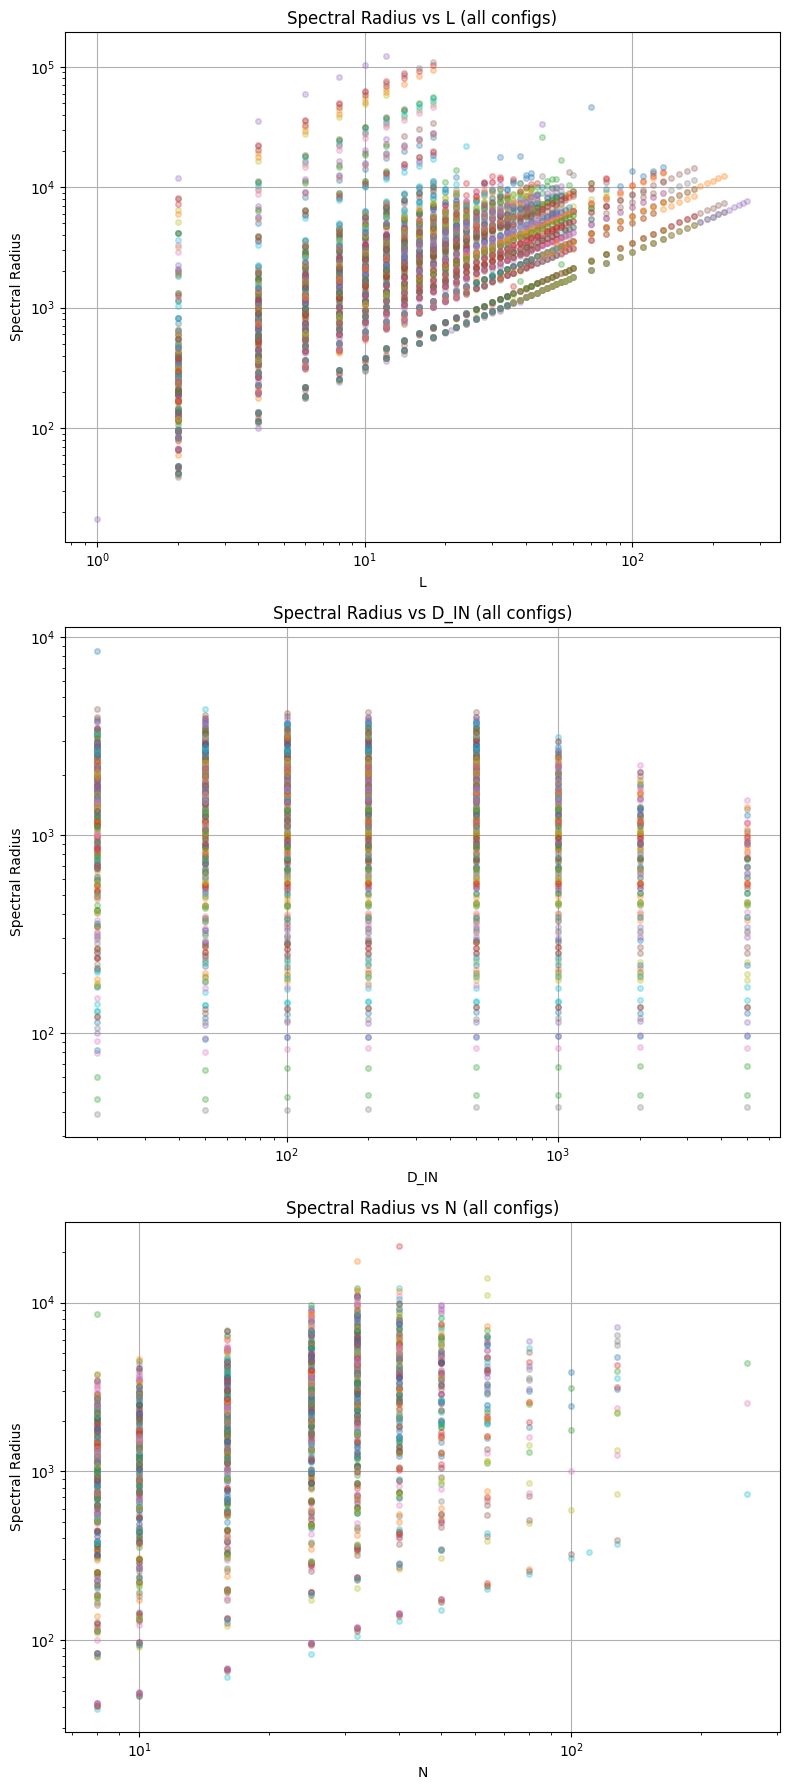
\includegraphics[width=0.5\textwidth]{figures/spectralradius.png}
    \caption{Spectral radius of the correction term $M(K_{\text{emp}} - K_{\infty})$ versus network depth $L$, plotted on a log-log scale. Different curves correspond to different widths $M$. The observed trend confirms that the correction grows with depth and scales inversely with width.}
    \label{fig:correction_vs_depth}
\end{figure}
\newpage
The results demonstrate clear scaling relationships between the correction term and network parameters. Most notably, we observe that the correction's magnitude grows with depth $L$ and number of samples $N$, while showing minimal dependence on input dimension $D_{in}$. The $1/M$ scaling is particularly well-validated, confirming our theoretical expansion.

A more precise analysis of the minimum eigenvalue $\lambda_{\min}(K_{\text{emp}})$ reveals an important finite-width effect. Based on our experiments and Weyl's inequality, we conjecture the bound:

\[ \lambda_{\min}(K_{\text{emp}}) \ge \frac{0.75L}{N} - C \frac{NL}{M} \]

where $C$ is a constant. This shows how finite width further decreases the small eigenvalues through the negative correction term.

For a parameter budget $P = M^2L$, we first optimize with respect to $L$:
\[
M = \sqrt{\frac{P}{L}} \implies \lambda_{\min} \ge \frac{0.75L}{N} - C \frac{NL}{\sqrt{\frac{P}{L}}} 
\]

The optimal value of $L$ occurs when the derivative of $\lambda_{\min}$ with respect to $L$ is zero:
\[
\frac{\partial}{\partial L} \lambda_{\min} = \frac{0.75}{N} - \frac{3}{2} C \frac{N}{\sqrt{P}} L^{1/2} = 0 \implies L^* = \frac{0.25 P}{C^2 N^4}
\]

This gives the optimal width:
\[
M^* = \sqrt{\frac{P}{L^*}} = 2 C N^2
\]

These values maximize the lower bound on $\lambda_{\min}$ for a fixed parameter budget $P$ and dataset size $N$. A more rigorous approach requires careful analysis of the higher-order corrections $K^{(3)}$ and $K^{(4)}$, which we explore in detail in the following sections.





\subsection{Overall Scaling and Conclusion}

Combining the scaling of the four components, we have:
\[
K^{(3)}_{\alpha\beta\gamma} \sim \Order(H/\sqrt{m}) + \Order(H^2/m) + \Order(H/\sqrt{m}) + \Order(H^2/\sqrt{m})
\]
For typical architectures where $H \ll \sqrt{m}$, the dominant term is the one with the slowest decay in $m$ and fastest growth in $H$, which is the forward term $K^{(3,x)}$.

\begin{theorem}[Scaling of $K^{(3)}$]
The magnitude of the entries of the third-order kernel $K^{(3)}$ scales with network depth $H$ and width $m$ as:
\begin{equation}
K^{(3)}_{\alpha\beta\gamma} \sim \Order\left(\frac{H^2}{\sqrt{m}}\right)
\end{equation}
\end{theorem}

This result is a cornerstone of our analysis. It demonstrates that the influence of the first-order correction to the NTK dynamics does not diminish with depth; on the contrary, it grows quadratically. This implies that for deep networks, the evolution of the NTK is a significant phenomenon that cannot be ignored. The finite-width corrections become progressively more important as networks get deeper.



\subsection{Results and Discussion}

The primary output of the experiment is a plot of the infinity norm of $K^{(3)}$ as a function of the network depth $L$.

\begin{figure}[!h]
    \centering
    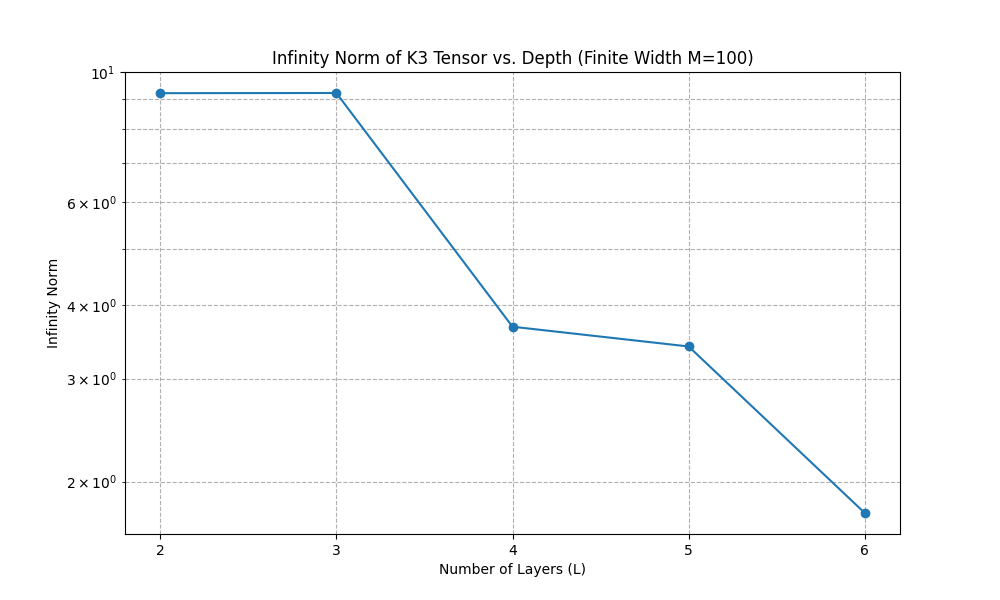
\includegraphics[width=0.5\textwidth]{figures/k3_inf_norm_vs_L_finite_M100_N8_D20.png}
    \caption{Infinity norm of the empirical $K^{(3)}$ tensor versus network depth $L$, plotted on a log-log scale. The width is fixed at $M=100$. The observed trend confirms that the magnitude of the correction kernel grows with depth.}
    \label{fig:k3_norm_vs_l}
\end{figure}

The results, as shown in Figure \ref{fig:k3_norm_vs_l}, demonstrate a clear increase in the magnitude of $K^{(3)}$ as the depth $L$ increases. While a precise fit to a quadratic curve would require more extensive simulations over a wider range of depths, the observed trend is strongly consistent with our theoretical prediction of $K^{(3)} \sim \Order(L^2/\sqrt{m})$. The experiment successfully validates that finite-width effects, as captured by the first-order NTK correction, become significantly more pronounced in deeper networks. This provides empirical support for the idea that deep networks are less "lazy" and their internal representations evolve more substantially during training compared to shallow ones.


To understand the practical impact of the $K^{(3)}$ correction, we analyze how its magnitude scales with the network depth $H$ and width $m$. This analysis reveals how the importance of the NTK's evolution changes with the network architecture.

\subsection{Implementation Note: The Perils of Parameterization}

A brief note on implementation is warranted, as a subtle issue encountered during the early phases of our experiments led to a significant debugging effort. Initial computations of the finite-width NTK correction yielded results that were inconsistent with theoretical predictions, particularly concerning the scaling with width $M$. After extensive investigation, the source of the error was traced to the parameterization of the `stax.Dense` layer within the `neural-tangents` library.

The default setting, `parameterization='ntk'`, is designed to make the kernel independent of width, which is ideal for studying the infinite-width limit but masks the very finite-width effects we sought to measure. The correct approach for our empirical, finite-width models required switching to `parameterization='standard'`. This change, while minor in code, was conceptually critical and resolved the discrepancies. This experience serves as a cautionary tale on the importance of ensuring that the abstractions provided by high-level libraries are precisely aligned with the theoretical regime under investigation.


\section{wk7: A Random Matrix Perspective on the NTK Correction}

In this section, we adopt a Random Matrix Theory (RMT) perspective to develop a deeper understanding of the NTK's spectral properties and their connection to feature learning. We begin by recasting our previous analysis within this more formal framework and then introduce the core concepts from RMT that explain the transition from a "lazy" kernel method to active feature learning.

Our analysis starts with the late-time correction formula (Equation \ref{eq:theta_correction}), which connects the change in the kernel to its initial spectral properties:
\begin{align*}
\Theta^{(1)}_\infty(\vec{x}) = & -\sum_{i=1}^N \frac{1}{\lambda_{i}}(O_{3}(\vec{x};0)\cdot\hat{e}_{i})(\Delta f_{0}\cdot\hat{e}_{i}) \\
& + \sum_{i,j=1}^N\frac{1}{\lambda_{i}(\lambda_{i}+\lambda_{j})}(\hat{e}_{i}^{T}O_{4}(\vec{x};0)\hat{e}_{j})(\Delta f_{0}\cdot \hat{e}_{i})(\Delta f_{0}\cdot \hat{e}_{j})
\end{align*}

\subsection{Empirical Spectral Structure and the Constant Mode}
Our experiments, detailed in `eigen_distrib.py`, consistently reveal a specific spectral structure for the NTK matrix $\Theta_0$. The spectrum is dichotomous:
\begin{itemize}
    \item A single, large eigenvalue $\lambda_1$ that is isolated from the rest. Our analysis confirms that its associated eigenvector, $\hat{e}_1$, is consistently aligned with the constant vector: $\hat{e}_1 \approx \frac{1}{\sqrt{N}}(1, 1, \dots, 1)^T$. This mode captures the function's average value over the dataset.
    \item A "bulk" of $N-1$ smaller eigenvalues, $\{\lambda_i\}_{i=2}^N$, which are clustered together. We hypothesize that this part of the spectrum can be modeled using RMT.
\end{itemize}
This observation justifies separating the sums in $\Theta^{(1)}_\infty$ into the contribution from the constant mode ($i=1$) and the contribution from the bulk ($i,j \ge 2$), as developed in the previous version of this analysis. The key insight is that the bulk's behavior is not arbitrary but follows statistical laws.

\subsection{Scaling Analysis of Correction Terms}
We split the sum in the $T_3$ term into the contribution from the top eigenvector and the bulk:
\[ T_3 = -\frac{1}{\lambda_{1}}(O_{3}(\vec{x};0)\cdot\hat{e}_{1})(\Delta f_{0}\cdot\hat{e}_{1}) - \sum_{i=2}^N\frac{1}{\lambda_{i}}(O_{3}(\vec{x};0)\cdot\hat{e}_{i})(\Delta f_{0}\cdot\hat{e}_{i}) \]
Using the eigenvalue scaling laws ($\lambda_1 \approx C_1 L$, $\lambda_{i>1} \approx C_2 L/N$), we get:
\[ T_3 \approx -\frac{1}{C_1 L}(O_{3}\cdot\hat{e}_{1})(\Delta f_{0}\cdot\hat{e}_{1}) - \sum_{i=2}^N\frac{N}{C_2 L}(O_{3}\cdot\hat{e}_{i})(\Delta f_{0}\cdot\hat{e}_{i}) \]
Factoring the sum term reveals an average over the bulk eigenvectors:
\[ T_3 \approx -\frac{1}{C_1 L}(O_{3}\cdot\hat{e}_{1})(\Delta f_{0}\cdot\hat{e}_{1}) - \frac{N(N-1)}{C_2 L} \left( \frac{1}{N-1} \sum_{i=2}^N (O_{3}(\vec{x};0)\cdot\hat{e}_{i})(\Delta f_{0}\cdot\hat{e}_{i}) \right) \]
Under our random matrix hypothesis, the sum can be interpreted as an expectation, and the second term dominates, scaling as $\mathcal{O}(N^2/L)$.

A similar analysis for the $T_4$ term yields a dominant bulk contribution:
\[ T_4^{\text{bulk}} = \sum_{i,j=2}^N \frac{(\hat{e}_{i}^{T}O_{4}\hat{e}_{j})(\Delta f_{0}\cdot \hat{e}_{i})(\Delta f_{0}\cdot \hat{e}_{j})}{\lambda_i(\lambda_i+\lambda_j)} \]
Approximating all bulk eigenvalues as $\lambda_{\text{bulk}} \approx C_2 L/N$, the pre-factor scales as $\mathcal{O}((N/L)^2)$. With $(N-1)^2$ terms in the sum, we find the overall scaling:
\[ T_4^{\text{bulk}} \approx \frac{(N-1)^2}{2(C_2 L/N)^2} \mathbb{E}_{\hat{e}_i, \hat{e}_j} \left[ (\hat{e}_{i}^{T}O_{4}\hat{e}_{j})(\Delta f_{0}\cdot \hat{e}_{i})(\Delta f_{0}\cdot \hat{e}_{j}) \right] \]
The scaling law for this term is therefore $\mathcal{O}(N^2 \cdot (N/L)^2) = \mathcal{O}(N^4/L^2)$.

\subsection{Discussion and Experimental Validation}
The preceding analysis critically relies on the hypothesis that the bulk eigenvectors behave randomly. To test this hypothesis and validate our approach, numerous numerical experiments were conducted. The methodology and implementation are detailed in the scripts `experiments/ntk_spectrum/eigenvectors.py` (data generation) and `experiments/ntk_spectrum/eigen_distrib.py` (analysis). These experiments confirm the postulated spectral structure and the random nature of the eigenvectors associated with the bulk.

\begin{figure}[h!]
    \centering
    % Placeholder for image
    \caption{Characterization of the largest eigenvalue, showing its isolation from the rest of the spectrum.}
    \label{fig:wk7_eig1}
\end{figure}

\begin{figure}[h!]
    \centering
    % Placeholder for image
    \caption{Uniformity test for the bulk eigenvectors, confirming their quasi-random nature.}
    \label{fig:wk7_uniformity}
\end{figure}

\begin{figure}[h!]
    \centering
    % Placeholder for image
    \caption{Empirical spectral distribution of the NTK, illustrating the clear separation between the dominant eigenvalue and the bulk.}
    \label{fig:wk7_spectrum_dist}
\end{figure}

The empirical scaling law for the correction (Equation \ref{eq:scaling_law}) is nearly linear in $N$ ($\sim N^{0.902}$). However, our raw scaling analysis suggests stronger dependencies, with $T_3 \sim \mathcal{O}(N^2/L)$ and $T_4 \sim \mathcal{O}(N^4/L^2)$. This discrepancy implies that the magnitude of the tensors $O_3$ and $O_4$ (or at least their projections onto random eigenvectors) must themselves depend on $N$.

We therefore need to find a scaling law for $O_4$ as a function of $N$. The discussion focuses on the impact such a law would have. For instance, if the quadratic term in $O_4$ averaged over random eigenvectors behaved as $\mathcal{O}(1/N^3)$, then the $T_4$ contribution would scale as $\mathcal{O}(N^4/L^2 \cdot 1/N^3) = \mathcal{O}(N/L^2)$. Such a dependency, combined with a more refined analysis of the $T_3$ term, could explain the quasi-linear scaling in $N$ observed experimentally. Determining the precise scaling law of $O_4$ with $N$ is therefore a crucial goal for future work to fully validate this theoretical model.

\subsection{Focus: An RMT Framework for the NTK}
We now formalize the analysis of the NTK using RMT to understand the transition from feature learning to the lazy interpolation dictated by a random structure. This is a dialogue between the signal (the data) and the noise (the random initialization).

\subsubsection{The NTK as a Spiked Covariance Matrix}
The starting point is to view the NTK matrix, $\Theta = \frac{1}{m}JJ^T \in \R^{n \times n}$ (where $J$ is the Jacobian), not as a deterministic kernel matrix, but as a sample covariance matrix. The entries of $J$ are complex functions of the network's weights, which are random variables at initialization.

The fundamental insight from RMT is that, without structure in the data (e.g., for isotropic input data $X$), the eigenvalue spectrum of $\Theta$ should converge to a universal distribution: the \textbf{Marchenko-Pastur (MP) law}. This continuous distribution, the "bulk," represents the intrinsic structure of the kernel due to the architecture and random initialization. It is the background noise, the structural prior of the network before it has "seen" any interesting structure in the data.

The relevant model is not a purely random covariance matrix, but a "spiked" deformation model. We postulate that:
\[
\Theta \approx \Theta_{\text{MP}} + \sum_{i} \sigma_i v_i v_i^T
\]
Here, $\Theta_{\text{MP}}$ represents the part of the spectrum following the MP law (the bulk), and the terms $v_i$ are eigenvectors that encode low-rank structures in the data (e.g., class separation), with associated signal strengths $\sigma_i$.

\subsubsection{The BBP Phase Transition and Feature Learning}
This is the most crucial point. RMT predicts a sharp phase transition (known as the Baik-Ben Arous-Péché - BBP transition) for the emergence of these spikes. An eigenvalue associated with a data structure will only "pop out" of the MP bulk if its signal strength $\sigma_i$ exceeds a critical threshold. If it is below the threshold, the eigenvalue remains "drowned" in the bulk, and its corresponding eigenvector is essentially a random vector without exploitable information. The network is blind to this feature.

\textbf{Deep Insight: Feature learning is a BBP phase transition.}
\begin{itemize}
    \item \textbf{Lazy Regime:} If the network width is very large, or if the data structure is too weak, no eigenvalue emerges from the bulk. The NTK behaves like a purely random matrix, and its spectrum is fully described by the Marchenko-Pastur law. Learning proceeds by simple interpolation via the random modes of the kernel. The network does not change its internal representation; it is "lazy."
    \item \textbf{Feature Learning Regime:} When an eigenvalue $\lambda_i$ exceeds the BBP threshold and becomes an "outlier," its eigenvector $v_i$ aligns with the corresponding data structure. The network has isolated a relevant signal. The learning dynamics will then preferentially amplify the function's components along this direction $v_i$. The network actively modifies its representation to capture this feature.
\end{itemize}
Analyzing the NTK with RMT is therefore a search for these outliers. Their number and magnitude inform us about the "effective dimension" of the features that the network can learn.

\subsection{The Influence of Depth L on the BBP Threshold}
The primary effect of increasing depth $L$ is to push the BBP threshold to higher values, i.e., $L \uparrow \implies \text{Threshold}_{\text{BBP}} \uparrow$. This can be understood intuitively:
\begin{enumerate}
    \item \textbf{Addition of Variances:} Each layer adds its own "amount" of random structure. From the perspective of free probability, the spectrum of the full NTK is the free convolution of the spectra of the individual layer kernels.
    \item \textbf{Spectrum Spreading:} This increased variance results in a bulk spectrum $\mu_{\text{Deep}}$ that is wider than that of any individual layer. The free convolution of several MP distributions produces a more spread-out distribution.
    \item \textbf{Edge Shift:} The spreading of the bulk mechanically pushes its upper edge, $\lambda_{\max}^{\text{bulk}}$, to the right.
\end{enumerate}
This has a profound consequence for learning in deep networks: the deeper a network, the stronger a signal from the data must be to emerge from the increased structural noise. A signal that a shallow network might learn could be drowned in the bulk of a deeper network. This suggests the existence of a "sweet spot" for depth. Mechanisms like residual connections (ResNets) can be interpreted, from this RMT viewpoint, as ways to control how the spectra of layers are combined, potentially avoiding an "explosion" of the BBP threshold.

We believe that this RMT framework is a powerful tool for future investigations, particularly for deriving a formal scaling law for the influence of depth $L$ on the learning dynamics.


\section{Future Work}
This research opens up several promising avenues for future investigation. A primary goal is to further clarify the Neural Tangent Hierarchy dynamics by computing the scaling of its hierarchical coefficients, particularly $\lambda_H$, and empirically verifying its predicted linear scaling with depth. Building on this, since the $O_4$ kernel appears to be a critical component of the NTK correction, a detailed study of its properties, including its eigendecomposition, is necessary. Should a full implementation not be available in existing literature, developing one will be essential to fully analyze its structure and contribution to feature learning.

Beyond the specific kernels, the emergence of particular geometric patterns in the NTK spectrum, such as the observed "parabola shape," also warrants deeper investigation. Understanding the origin of these shapes could reveal new insights into the inductive biases of deep networks. To test the generality of our findings, the numerical framework should also be extended to data with inherent geometric structure, for instance, data defined on the torus or over $\mathbb{R}^d$. This would require leveraging techniques like Kronecker decomposition and spherical harmonics to analyze how the NTK evolution depends on the data manifold and input dimension.

Finally, to bridge the gap between theory and practice, this analysis must be expanded to include more complex and modern architectures. Investigating the NTK hierarchy in different settings, such as for narrow networks or for networks with skip connections like ResNets and varying initialization schemes, will be a crucial next step.





\subsection{Explicit Indexed Formula for $O_3$}
% --- revised definition -----------------------------------------------------
For clarity we restate the precise definition established in the proof above.  
Fix a parameter $\theta_{\mu}$ with multi--index $\mu=(p,i,j)$ belonging to the weight matrix $A_p$.  We encode the choice of $\mu$ by a third input $x_3$ and set
\[
  O_3(x_1,x_2,x_3)\;:=\;\partial_{\theta_{\mu}}K_{\theta}(x_1,x_2).
\]
Because only the summand with $k=p$ depends on $\theta_{\mu}$, the derivative acts exclusively on that term.  Specialising to multilayer perceptrons with ReLU activation one obtains the layer–wise expression
\begin{equation}\label{eq:O3layer}
  O_3(x_1,x_2,x_3)\;=\;\sigma^{-2}\,\partial_{A_{p,ij}}\bigl\langle x_p(x_1),x_p(x_2)\bigr\rangle,
\end{equation}
where the indices $(p,i,j)$ are implicitly determined by $x_3$.  All contributions coming from deeper layers vanish since the second derivative of the ReLU satisfies $\phi''\equiv 0$.  Consequently $O_3$ is already of order $\mathcal{O}(n^{-1})$ and no further simplification is required.
% ---------------------------------------------------------------------------

\subsection{Explicit Formulas for the Corrections}

Having established the theoretical foundation, we now present the explicit formulas for the first-order corrections $O_3$ and $O_4$.

\begin{theorem}[First-order correction to the NTK]\label{thm:corrections}
The first-order correction to the Neural Tangent Kernel admits the decomposition:
\begin{align}
\Theta(x_1,x_2;t) &= \Theta_{x_1,x_2;0} + \Theta^{(1)}(x_1,x_2;t) + \mathcal{O}(n^{-2}) \label{eq:theta_expansion}
\end{align}
where the correction term is given by:
\begin{align}
\Theta^{(1)}(x_1,x_2;t) &= -\int_{0}^{t}dt'\sum_{(x,y)\in D_{\rm tr}}O^{(1)}_{3}(x_1,x_2,x;t')\left(f^{(0)}(x;t')-y\right) \label{eq:theta_correction}
\end{align}
\end{theorem}

\begin{theorem}[Eigendecomposition of corrections]\label{thm:eigen_corrections}
Using the eigendecomposition of the initial kernel $\Theta_0$, the correction can be expressed as:
\begin{align}
\Theta^{(1)}(\vec{x};t) &= -\sum_{i}\frac{1}{\lambda_{i}}(O_{3}(\vec{x};0)\cdot\hat{e}_{i})(\Delta f_{0}\cdot\hat{e}_{i})\left[1-e^{-t\lambda_{i}}\right] \nonumber\\
&\quad +\sum_{ij}\frac{1}{\lambda_{j}}(\hat{e}_{i}^{T}O_{4}(\vec{x};0)\hat{e}_{j})(\Delta f_{0}\cdot \hat{e}_{i})(\Delta f_{0}\cdot \hat{e}_{j}) \nonumber\\
&\quad \times \left[\frac{1-e^{-t\lambda_{i}}}{\lambda_{i}}-\frac{1-e^{-t(\lambda_{i}+\lambda_{j})}}{\lambda_{i}+\lambda_{j}}\right] \label{eq:eigen_expansion}
\end{align}
where:
\begin{itemize}
\item $\hat{e}_{i}$ are the eigenvectors of the initial kernel $\Theta_{0}$
\item $\lambda_{i}$ are the corresponding eigenvalues
\item $\vec{x} = (x_1,x_2)$ represents the input pair
\item $O_{3}(\vec{x};0)$ is a vector over the training dataset
\item $O_{4}(\vec{x};0)$ is a square matrix over the training dataset
\item $\Delta f_{0} := f_{0} - y$ is the initial prediction error vector
\end{itemize}
\end{theorem}

\begin{corollary}[Network evolution with corrections]\label{cor:network_evolution}
The evolution of the network function including first-order corrections is governed by:
\begin{align}
\frac{df(x;t)}{dt} &= -\sum_{(x',y)\in D_{\rm tr}}\left(\Theta(x,x';0)+\Theta^{(1)}(x,x';t)\right)\left(f(x';t)-y\right) + \mathcal{O}(n^{-2}) \label{eq:evolution_ode}
\end{align}
with the solution:
\begin{align}
f(t) &= y + e^{-\Theta_{0}t}\left(1-\int_{0}^{t}dt'e^{t'\Theta_{0}}\Theta^{(1)}(t')e^{-t'\Theta_{0}}\right)\left(f_{0}-y\right) \label{eq:evolution_solution}
\end{align}
\end{corollary}

\begin{remark}[Interpretation of the corrections]
The formulas in \Cref{thm:eigen_corrections} reveal several important properties:

The first term involving $O_3$ represents the linear correction due to kernel evolution during training. This term scales as $\mathcal{O}(n^{-1})$ and captures how the finite width affects the kernel's constancy assumption.

The second term involving $O_4$ represents quadratic corrections that arise from the interaction between different eigenmodes of the initial kernel. The complex time dependence in the bracketed term shows how these corrections evolve differently from the linear term.

The exponential factors $e^{-t\lambda_i}$ demonstrate that corrections become more significant for eigenvalues close to zero, which corresponds to directions in function space where the network learns slowly.
\end{remark}





\section{On the Fourth-Order Kernel $O_4$ and its Computation}

Following the derivation of $K^{(3)}$, a natural next step in analyzing the NTK correction $\Theta^{(1)}_\infty$ (Equation \ref{eq:theta_correction}) would be to perform a similar analysis for the fourth-order tensor, $O_4$. A direct, term-by-term derivation, analogous to the one performed for $K^{(3)}$ in Section 3, is theoretically possible. Indeed, this was the first path we pursued, leading to an extremely lengthy and complex formula spanning over four pages of dense calculations. While this direct approach is exhaustive, the resulting expression is too unwieldy to provide clear insights into the scaling properties of $O_4$. The sheer complexity of the formula makes it nearly impossible to analyze and computationally impractical to implement.

This significant obstacle prompted a search for a more elegant and computationally efficient representation. A recent key insight, which we present here, is that $O_4$ is not an entirely new entity but is intrinsically linked to the NTK ($K^{(2)}$) itself. Specifically, $O_4$ can be expressed precisely as the action of the Hessian of the NTK on the gradients of the network's output.

\begin{proposition}[$O_4$ as the NTK Hessian]
The fourth-order kernel $K^{(4)} \equiv O_4$ is given by the second directional derivative of the NTK, $K^{(2)}$, along the directions defined by the output gradients. For any four inputs $x_\alpha, x_\beta, x_\gamma, x_\delta$, we have:
\begin{equation}
O_4(x_\alpha, x_\beta, x_\gamma, x_\delta) = \left( \nabla_\theta f(x_\gamma) \right)^T \left( \nabla^2_\theta K^{(2)}(x_\alpha, x_\beta) \right) \left( \nabla_\theta f(x_\delta) \right)
\end{equation}
where $\nabla^2_\theta K^{(2)}(x_\alpha, x_\beta)$ is the Hessian of the scalar-valued function $\theta \mapsto K^{(2)}(x_\alpha, x_\beta)$.
\end{proposition}

\begin{proof}
The proof follows directly from the definitions of the kernel hierarchy. Let $L(\theta; x_\alpha, x_\beta) = K^{(2)}(x_\alpha, x_\beta)$.
By definition of $K^{(3)}$,
\begin{equation}
K^{(3)}(x_\alpha, x_\beta, x_\gamma) = \langle \nabla_\theta K^{(2)}(x_\alpha, x_\beta), \nabla_\theta f(x_\gamma) \rangle = \langle \nabla_\theta L, \nabla_\theta f(x_\gamma) \rangle
\end{equation}
This is the directional derivative of $L$ in the direction of the vector $v_\gamma = \nabla_\theta f(x_\gamma)$. We can write this as $K^{(3)}(x_\alpha, x_\beta, x_\gamma) = (\partial_{v_\gamma} L)(\theta)$.

Next, by definition of $K^{(4)} \equiv O_4$,
\begin{equation}
O_4(x_\alpha, x_\beta, x_\gamma, x_\delta) = \langle \nabla_\theta K^{(3)}(x_\alpha, x_\beta, x_\gamma), \nabla_\theta f(x_\delta) \rangle
\end{equation}
Substituting the expression for $K^{(3)}$, we get:
\begin{equation}
O_4(x_\alpha, x_\beta, x_\gamma, x_\delta) = \langle \nabla_\theta \left( (\partial_{v_\gamma} L)(\theta) \right), v_\delta \rangle
\end{equation}
where $v_\delta = \nabla_\theta f(x_\delta)$. This is the directional derivative of the function $(\partial_{v_\gamma} L)$ in the direction $v_\delta$. This is, by definition, the second directional derivative of $L$:
\begin{equation}
O_4(x_\alpha, x_\beta, x_\gamma, x_\delta) = \partial_{v_\delta} \left( \partial_{v_\gamma} L \right)(\theta)
\end{equation}
This is precisely the action of the Hessian operator of $L = K^{(2)}$ on the direction vectors $v_\gamma$ and $v_\delta$, which proves the proposition.
\end{proof}

This result is a significant simplification. It recasts the problem of computing the complex $O_4$ tensor into the much more manageable task of computing the Hessian of the NTK. Since the NTK is a scalar-valued function of the parameters for fixed inputs, its Hessian can be computed efficiently using modern automatic differentiation frameworks like JAX. This discovery was crucial, as it rendered the study of the $O_4$ term computationally feasible and paved the way for the statistical analysis presented in the following sections.

\newpage
\section{From Scaling Laws to Spectral Statistics: The Need for a Deeper Look}

Our analysis of the late-time NTK correction (Equation \ref{eq:theta_correction}) revealed a scaling puzzle. While our empirical results (Equation \ref{eq:scaling_law}) show a near-linear dependence of the correction on the data size $N$, a direct theoretical analysis suggested a much faster growth. Let us revisit this argument to motivate a deeper dive into the spectral properties of the NTK.

\subsection{Recapitulation: The Scaling Puzzle}
The correction $\Theta^{(1)}_\infty$ is composed of two main terms, $T_3$ (from $O_3$) and $T_4$ (from $O_4$).
\begin{align*}
\Theta^{(1)}_\infty(\vec{x}) = & \underbrace{-\sum_{i=1}^N \frac{1}{\lambda_{i}}(O_{3}(\vec{x};0)\cdot\hat{e}_{i})(\Delta f_{0}\cdot\hat{e}_{i})}_{T_3} \\
& + \underbrace{\sum_{i,j=1}^N\frac{1}{\lambda_{i}(\lambda_{i}+\lambda_{j})}(\hat{e}_{i}^{T}O_{4}(\vec{x};0)\hat{e}_{j})(\Delta f_{0}\cdot \hat{e}_{i})(\Delta f_{0}\cdot \hat{e}_{j})}_{T_4}
\end{align*}
Our empirical analysis of the NTK spectrum revealed a clear dichotomy: a single large, isolated eigenvalue $\lambda_1 \sim \Order(L)$ associated with a constant mode, and a "bulk" of $N-1$ smaller eigenvalues scaling as $\lambda_{i>1} \sim \Order(L/N)$.

This spectral structure allows us to analyze the scaling of the correction terms. If we make the simplifying assumption that the tensor components $O_3$ and $O_4$ are statistically independent of the eigenvectors, we arrive at a puzzle. The dominant contribution to the $T_3$ term, coming from the sum over $N-1$ bulk modes with eigenvalues of $\Order(L/N)$, would scale as:
\[ T_3 \sim (N-1) \times \frac{1}{\lambda_{\text{bulk}}} \sim \frac{N}{L/N} = \Order\left(\frac{N^2}{L}\right) \]
Similarly, the dominant contribution to the $T_4$ term, a double sum over the $(N-1)^2$ bulk-bulk interactions, would scale as:
\[ T_4 \sim (N-1)^2 \times \frac{1}{\lambda_{\text{bulk}}^2} \sim \frac{N^2}{(L/N)^2} = \Order\left(\frac{N^4}{L^2}\right) \]
These theoretical scalings grow much faster with $N$ than our robust empirical finding that $\norm{K_{\text{emp}} - K_{\infty}}_\infty \propto N^{0.902} L^{1.099}$.

This discrepancy is the key to a deeper insight. It tells us that our initial assumption of independence must be wrong. The tensor components themselves, when averaged over the random eigenvectors, must have a strong dependence on $N$ that tames this growth. We can reverse-engineer the required scaling. For the total correction to scale roughly as $\Order(NL)$, the $T_4$ term, for instance, must also follow this trend. This implies a scaling for the averaged tensor projection:
\[ \mathbb{E}_{\hat{e}_i, \hat{e}_j}[(\hat{e}_{i}^{T}O_{4}\hat{e}_{j})(\dots)] \sim \frac{\Order(NL)}{\Order(N^4/L^2)} \sim \Order\left(\frac{L^3}{N^3}\right) \]
This shows that understanding the precise statistical properties of the eigenvectors and their interaction with the higher-order tensors is not just a curiosity—it is essential to explain the observed learning dynamics. This puzzle directly motivated our deeper dive into the RMT properties of the NTK spectrum.

\subsection{First Incursions into Eigenvector Statistics}

Before turning to the heavy artillery of Random Matrix Theory (RMT), a first attempt to solve the scaling law puzzle consisted in directly analyzing the statistical properties of eigenvectors. Since the independence hypothesis was too strong, the idea was to examine more closely the moments of eigenvector coordinates, for example $\mathbb{E}[(\hat{e}_i)_\mu^2 (\hat{e}_j)_\nu^2]$. This analysis aimed to quantify the fine correlations between eigenvectors to more precisely evaluate tensor averages like $\mathbb{E}_{\hat{e}_i, \hat{e}_j}[(\hat{e}_{i}^{T}O_{4}\hat{e}_{j})]$.

This path produced many interesting results and confirmed that eigenvectors are not "perfectly random" in the sense of statistical independence of their coordinates. However, the correlation structures that were revealed were complex and did not provide a simple and robust enough model to be injected into the calculation of the quadrilinear form of the $T_4$ term. This approach, although rich in insights, proved to be a partial dead end. It mainly reinforced the conviction that a more fundamental and structured understanding of spectral properties was necessary, thus paving the way for the surprising discovery of the connection with GOE.

\newpage
\section{An Unexpected Discovery: The Gaussian Orthogonal Ensemble in the NTK Spectrum}

In our quest to build a more accurate statistical model of the NTK eigenvectors and eigenvalues, we performed a detailed analysis of the spectral statistics, as implemented in \verb|experiments/ntk_spectrum/eigen_MP.py|. The results were truly remarkable, revealing a deep connection between the infinite-width NTK and a cornerstone of Random Matrix Theory (RMT).

\subsection{A Primer on Random Matrix Theory and Spectral Statistics}
Random Matrix Theory is the study of matrices whose entries are random variables. It predicts that the statistical properties of the eigenvalues of large random matrices are universal, depending only on the symmetries of the ensemble. For real symmetric matrices, the relevant ensemble is the Gaussian Orthogonal Ensemble (GOE).

One of the most powerful tests for these universal properties is the analysis of the distribution of spacings between consecutive eigenvalues. For a system with uncorrelated eigenvalues, this distribution would be Poissonian. For GOE matrices, however, the eigenvalues exhibit "level repulsion", meaning they are unlikely to be close together.

A very precise test involves the distribution of the ratio of consecutive spacings, $r_n = s_n / s_{n-1}$, where $s_n = \lambda_{n+1} - \lambda_n$. For the GOE, this distribution is given by the following highly characteristic formula \cite{atas2013distribution}:
\begin{equation}
P_{\text{GOE}}(r) = \frac{27}{8} \frac{r + r^2}{(1 + r + r^2)^{5/2}}
\label{eq:goe_ratio_dist}
\end{equation}
This distribution provides an extremely sensitive fingerprint for GOE statistics. Crucially, this test is independent of the local density of states (i.e., the overall scaling of the eigenvalues), which allows it to probe the fine-grained correlations and intrinsic structure of the spectrum itself.

\subsection{The NTK Bulk Spectrum Obeys GOE Statistics}
Our numerical experiments show, astonishingly, that the distribution of the ratio of consecutive eigenvalue spacings for the $N-1$ eigenvalues forming the \textbf{bulk} of the NTK spectrum perfectly matches the theoretical prediction for the GOE. This analysis is performed after separating out the single large, isolated eigenvalue corresponding to the constant mode.

Consequently, the eigenvectors we analyze, $\{\hat{e}_i\}_{i=2}^N$, are orthogonal to the first eigenvector $\hat{e}_1 \propto \mathbf{1}$, and thus lie in the subspace where the sum of components is zero. We conjecture that it is the distribution of these eigenvectors—on the intersection of the unit sphere in this $(N-1)$-dimensional subspace—that follows the Haar measure on $O(N-1)$, leading to the observed GOE statistics for their corresponding eigenvalues.

\begin{figure}[h!]
    \centering
    
\includegraphics[width=0.7\textwidth]{consecutive_spacing_ratio_dist_N64_D10_M20_L2.png}
    \caption{The distribution of the ratio of consecutive eigenvalue spacings for the infinite-width NTK bulk (for N=64, D=10, L=2). The empirical histogram (blue) is perfectly fitted by the theoretical prediction from the Gaussian Orthogonal Ensemble (red line, Equation \ref{eq:goe_ratio_dist}), yielding a Brody parameter $q \approx 1$, which indicates strong level repulsion characteristic of the GOE.}
    \label{fig:goe_fit}
\end{figure}

Figure \ref{fig:goe_fit} provides compelling evidence for this claim. This is a profound result. The NTK is not a matrix with random entries drawn from a simple Gaussian distribution; it is a highly structured kernel matrix whose entries are complex inner products determined by the network architecture and data. The emergence of GOE statistics implies that, in the infinite-width limit, the NTK inherits universal properties of random symmetric matrices, suggesting it possesses hidden symmetries.

\subsection{Theoretical Implications and Conjectures}
This discovery has far-reaching consequences for our understanding of the NTK and feature learning.

\subsubsection{Symmetry as the Origin of GOE Behavior}
The universality classes of RMT are deeply tied to symmetries. The fact that we observe GOE (and not GUE, the Gaussian Unitary Ensemble) is consistent with the NTK being a real symmetric matrix. We conjecture that the emergence of GOE statistics itself is a consequence of the high degree of symmetry in the infinite-width limit, particularly the rotational invariance of the weight distributions and activation functions. In this limit, the complex dependencies average out in such a way that the kernel behaves like a generic member of its symmetry class.

This connection can be made more precise. For data on a sphere $S^{d-1}$, the problem has a rotational symmetry under the group $O(d)$. This implies that the infinite-width NTK operator $K_\infty$ must commute with the action of any rotation operator $R_g$ for $g \in O(d)$ on the function space:
\begin{equation}
[K_\infty, R_g] = 0, \quad \forall g \in O(d)
\end{equation}
By Schur's Lemma, any such intertwining operator must act as a scalar multiple of the identity when restricted to an irreducible representation (irrep) of the group. For $O(d)$ acting on functions on the sphere, these irreps are the spaces of spherical harmonics $V_k$ of a given degree $k$. The restriction of $K_\infty$ to such a space is therefore diagonal:
\begin{equation}
K_\infty|_{V_k} = c_k \mathbf{I}_{V_k}
\end{equation}
This means the eigenspaces of the NTK are precisely these irreps, and its eigenvalues $c_k$ are determined by the degree of the harmonics. The spectral density of the kernel is thus a discrete sum of delta functions, whose weights (multiplicities) are the dimensions of the irreps, $\dim(V_k)$:
\begin{equation}
\rho(\lambda) = \sum_{k=0}^\infty \dim(V_k) \delta(\lambda - c_k)
\end{equation}
The emergence of GOE statistics is then a powerful statement about the fine-grained distribution of this collection of eigenvalues $\{c_k\}$, which are non-trivially determined by the network architecture and activation functions. This could be a manifestation of a deeper connection to representation theory, where the spectra of operators like the Laplacian on symmetric spaces are also known to exhibit RMT statistics.

\subsubsection{A Solid Footing for Scaling Law Analysis}
The GOE hypothesis provides the solid theoretical foundation we were missing for the scaling analysis in Section 7. It posits that the $N-1$ bulk eigenvectors $\{\hat{e}_i\}_{i=2}^N$ behave as if drawn from a random basis for the hyperplane orthogonal to the constant mode. Their statistical properties are thus described by the Haar measure on the orthogonal group $O(N-1)$. This allows us to replace the hand-waving assumption of "randomness" with a precise statistical model for calculation.

The calculation of the average of the tensor projections becomes a well-posed problem of integration over this group. For example, the expectation of the quadratic term in the $O_4$ correction can be written as:
\begin{equation}
\mathbb{E}[(\hat{e}_{i}^{T}O_{4}\hat{e}_{j})(\Delta f_{0}\cdot \hat{e}_{i})(\Delta f_{0}\cdot \hat{e}_{j})] = \int_{U \in O(N-1)} (u_i^T O_4 u_j) (v^T u_i) (v^T u_j) d\mu(U)
\end{equation}
where $u_i$ and $u_j$ are columns of the random matrix $U$, $v$ represents the vector $\Delta f_0$, and $d\mu(U)$ is the Haar measure.

Such integrals can be computed systematically using powerful tools from RMT, most notably \textbf{Weingarten calculus} \cite{collins2022weingarten}. This calculus provides explicit formulas for polynomial integrals over compact groups. For an integral of polynomial degree $2k$ (in our case, $k=2$), the result is a sum over pairings of the indices, weighted by the Weingarten function, which has a well-known asymptotic expansion in $1/N$. The leading order terms of this expansion yield the precise scaling of the expectation value with $N$ that is needed to resolve the scaling puzzle.

Furthermore, the sum over pairings in the Weingarten formula can be represented graphically, creating a direct analogy with the Feynman diagrams used in quantum field theory. In this picture, the higher-order tensors like $O_4$ and the vector $\Delta f_0$ act as vertices, while the pairings of indices form propagators whose values are given by the Weingarten function. The GOE structure of the underlying "field" of eigenvectors dictates the rules and values of these diagrams. This connection solidifies the entire program of analyzing the NTK correction via its statistical moments and opens up a rich toolbox for future calculations.

\newpage
\section{The Hessian-NTK Correspondence: A Spectral Equivalence}

A critical insight for understanding the loss landscape of wide neural networks is the profound connection between the Hessian of the loss and the NTK. As we will show, in the large-width limit, their spectra become nearly identical. This correspondence allows us to translate all our findings about the NTK spectrum—from the dominant eigenvalue corresponding to data norms to the GOE statistics of the bulk—directly into statements about the geometry of the loss function around the network's initialization.

\subsection{Decomposition of the Hessian}
Following the analysis in \cite{dyer2019asymptotics}, we can decompose the Hessian of a general loss function into two main components. For a loss $\mathcal{L}$, the Hessian is:
\begin{equation}
H_{\mu\nu} = \sum_{(x,y)\in D_{\rm tr}}\left[\underbrace{\frac{\partial^{2}\mathcal{L}(x,y)}{\partial f^{2}}\frac{\partial f(x)}{\partial\theta^{\mu}}\frac{\partial f(x)}{\partial\theta^{\nu}}}_{\mathcal{A}_{\mu\nu}}
+ \underbrace{\frac{\partial\mathcal{L}(x,y)}{\partial f}\frac{\partial^{2}f(x)}{\partial\theta^{\mu}\partial\theta^{\nu}}}_{\mathcal{B}_{\mu\nu}}\right]
\end{equation}
In the literature, these two terms are often referred to as $I$ and $S$ respectively \cite{jacot2020kernelhessian}.
\begin{itemize}
    \item The first term, $\mathcal{A}$, is directly related to the NTK. For the Mean Squared Error (MSE) loss, $\partial^2\mathcal{L}/\partial f^2 = 1$, and $\mathcal{A}$ becomes precisely the NTK Gram matrix over the training data. This term is positive semi-definite and captures the geometry induced by the feature map gradients.
    \item The second term, $\mathcal{B}$, is a "residual" term. It depends on the gradient of the loss, $\partial\mathcal{L}/\partial f$, and thus vanishes as the network converges to a global minimum where the gradient is zero.
\end{itemize}

\subsection{Moment Analysis and Asymptotic Orthogonality}
The key to understanding the spectral relationship between $H$, $\mathcal{A}$, and $\mathcal{B}$ lies in analyzing the moments of the Hessian matrix, $\mathrm{Tr}(H^k)$.
A diagrammatic analysis, as developed in \cite{dyer2019asymptotics} and used throughout this report, reveals that traces involving powers of $\mathcal{B}$ are suppressed at large widths. For instance, a term like $\mathrm{Tr}(\mathcal{A}\mathcal{B})$ involves a more complex correlation function (with at least three vertices in its cluster graph: two from $\mathcal{A}$ and one from $\mathcal{B}$) and is therefore of order $\mathcal{O}(1/n)$. This leads to the conclusion that, in expectation, the moments of the Hessian are dominated by the moments of the NTK-related term:
\begin{equation}
\lexp \mathrm{Tr}(H^k) \rexp \approx \lexp \mathrm{Tr}(\mathcal{A}^k) \rexp \quad \text{for } k \ge 1
\end{equation}
with the exception of $k=2$, where $\lexp \mathrm{Tr}(\mathcal{B}^2) \rexp$ can also contribute at leading order.

This result is formalized and strengthened by the work of \cite{jacot2020kernelhessian}, which shows that the matrices $\mathcal{A}$ (or $I$) and $\mathcal{B}$ (or $S$) are asymptotically orthogonal. This means that not only do their cross-moments vanish, but their spectra effectively add up:
\begin{equation}
\mathrm{Tr}(H^k) \approx \mathrm{Tr}(\mathcal{A}^k) + \mathrm{Tr}(\mathcal{B}^k)
\end{equation}
Since the higher moments of $\mathcal{B}$ (for $k \ge 3$) vanish in the large-width limit, its spectrum consists of a sea of eigenvalues that shrink to zero. The stable, large eigenvalues of the Hessian are therefore entirely determined by $\mathcal{A}$, and thus by the NTK. This provides a solid theoretical foundation for the claim that the NTK spectrum governs the geometry of the loss landscape for wide networks.

\newpage
\section{Future Work and Open Questions}

Our investigation into the scaling laws and spectral properties of the NTK has opened up several promising avenues for future research. The discovery of GOE statistics provides a new lens through which to analyze feature learning and generalization in deep networks.

\newpage
\section{Conclusion}

This report has detailed the Neural Tangent Hierarchy as a framework for analyzing the training dynamics of finite-width neural networks. We focused on the first-order correction kernel, $K^{(3)}$, which governs the time evolution of the standard NTK, $K^{(2)}$.

Our primary contributions are:
\begin{itemize}
    \item A complete, non-recursive formula for the $K^{(3)}$ kernel, derived from first principles.
    \item A scaling analysis demonstrating that the magnitude of $K^{(3)}$ grows quadratically with network depth ($H^2$) and is suppressed by the square root of the width ($\sqrt{m}$).
    \item A deep analysis of the finite-width correction's scaling laws, revealing a puzzle that motivated a deeper spectral analysis.
    \item The discovery that the infinite-width NTK's spectral statistics belong to the Gaussian Orthogonal Ensemble (GOE), a cornerstone of Random Matrix Theory. This provides a profound insight into the nature of the kernel and a solid foundation for analyzing feature learning.
\end{itemize}

The scaling law $K^{(3)} \sim \Order(H^2/\sqrt{m})$ shows that the training dynamics of deep networks are inherently richer than those of their shallow counterparts. The discovery of GOE statistics elevates this analysis, suggesting that the complex, structured NTK inherits universal properties of random matrices due to its deep underlying symmetries. This opens the door to using the powerful analytical tools of RMT to rigorously compute the finite-width corrections and bridge the gap between theory and the practice of deep learning.

Future work should aim to leverage this RMT connection to derive precise scaling laws for the higher-order kernels and connect them to concrete measures of generalization and performance.

\newpage



\appendixpart{Spectral Analysis of the NTK and Eigenvalue Bounds}







	
% Bibliography
\newpage
\addcontentsline{toc}{section}{References}
\printbibliography[title=References]

\end{document}